\documentclass[12pt,a4paper]{article}
\usepackage{listings,chngcntr}
\usepackage{hyperref}% http://ctan.org/pkg/hyperref
\usepackage{paralist}
\usepackage{enumitem}% http://ctan.org/pkg/enumitem
\usepackage{amssymb}
\usepackage{amsmath,amsfonts,bm}
\usepackage{amsthm}
\newtheorem{theorem}{Theorem}[section]
\newtheorem{corollary}{Corollary}[theorem]
\newtheorem{definition}[theorem]{Definition}
\newtheorem{proposition}[theorem]{Proposition}
\newtheorem{lemma}[theorem]{Lemma}
\usepackage{url}
\usepackage{algorithm}
\usepackage{algpseudocode}
\usepackage{indentfirst}
\usepackage[percent]{overpic}
\makeatletter
\def\BState{\State\hskip-\ALG@thistlm}
\makeatother
\usepackage{mathtools}
\usepackage{fancyhdr}
\pagestyle{fancy}
\theoremstyle{definition}
\usepackage{float}
\usepackage[utf8]{inputenc}
\usepackage{cleveref}
\crefname{section}{§}{§§}
\Crefname{section}{§}{§§}
\newcommand{\R}{\mathbb{R}}
 \usepackage{stmaryrd}
 \usepackage{graphicx}
 \usepackage{caption}
 \usepackage{subcaption}
 \usepackage[english]{babel}
\usepackage{color}
\newcommand{\hilight}[1]{\colorbox{yellow}{#1}}
\usepackage{soul}
\usepackage{tikz}
\usetikzlibrary{hobby,shapes,arrows,fit,calc,positioning} 
\newcommand\restr[2]{{% we make the whole thing an ordinary symbol
		\left.\kern-\nulldelimiterspace % automatically resize the bar with \right
		#1 % the function
		\vphantom{\big|} % pretend it's a little taller at normal size
		\right|_{#2} % this is the delimiter
}}

\usepackage{listings}
\usepackage{color}
\usepackage{graphicx, epstopdf}
\usepackage{listings}
\lstset{language=Python}
\renewcommand{\sectionautorefname}{\S}
\setlength{\topmargin}{0.0in}
\setlength{\oddsidemargin}{0.33in}
\setlength{\textheight}{9.0in}
\setlength{\textwidth}{6.0in}
\renewcommand{\baselinestretch}{1.25}
%\linespread{1.3}
\setlist[itemize]{noitemsep, topsep=0pt}
\definecolor{codegreen}{rgb}{0,0.6,0}
\definecolor{codegray}{rgb}{0.5,0.5,0.5}
\lstset{
	frame=single,
	numbers = left,
	basicstyle=\fontsize{9}{11}\ttfamily\linespread{0.85}\ttfamily,
    breaklines=true
}



\begin{document}
	\begin{titlepage} % Suppresses headers and footers on the title page
		\centering % Centre everything on the title page
		\scshape % Use small caps for all text on the title page
	%	\vspace*{\baselineskip} % White space at the top of the page
		%------------------------------------------------
		%	Title
		%------------------------------------------------
		\rule{\textwidth}{1.6pt}\vspace*{-\baselineskip}\vspace*{2pt} % Thick horizontal rule
		\rule{\textwidth}{0.4pt} % Thin horizontal rule
	%	\vspace{0.75\baselineskip} % Whitespace above the title
		
		{\LARGE Hierarchical\ Model\\ Adaptivity\\} % Title
		
		\vspace{0.75\baselineskip} % Whitespace below the title
		
		\rule{\textwidth}{0.4pt}\vspace*{-\baselineskip}\vspace{3.2pt} % Thin horizontal rule
		\rule{\textwidth}{1.6pt} % Thick horizontal rule
		
		%\vspace{2\baselineskip} % Whitespace after the title block
		
		%------------------------------------------------
		%	Subtitle
		%------------------------------------------------
	%	A Number of Fascinating and Life-changing Templates Presented in a Clear and Concise Way % Subtitle or further description
		
		%\vspace*{1\baselineskip} % Whitespace under the subtitle
		
		%------------------------------------------------
		%	Editor(s)
		%------------------------------------------------
		

		
		\vspace{0.5\baselineskip} % Whitespace before the editors
		
		{\scshape\Large Author:\\ Georgios Sialounas \\$\,$\\ Supervisors: \\Dr Tristan Pryer\\Dr Oliver Sutton} % Editor list
		
	%	\vspace{0.5\baselineskip} % Whitespace below the editor list
		
	%	\textit{The University of Reading\\} % Editor affiliation
		
		\vfill % Whitespace between editor names and publisher logo
		
		
		%------------------------------------------------
		%	Publisher
		%------------------------------------------------
		
		\begin{figure}[H]
			\begin{subfigure}[b]{.15\linewidth}
				
\includegraphics[width=\linewidth]{icl_logo_big}
			%	\caption{Velocity in $L^2$: $\left|\left|u-u_h\right|\right|_{L^2}$.}
				\label{icl_logo_big}
			\end{subfigure}
			\begin{subfigure}[b]{.1263\linewidth}
				
\includegraphics[width=\linewidth]{uor_logo_big}
			%	\caption{Velocity in $H^1$: $\left|\left|u-u_h\right|\right|_{H^1}$.}
				\label{uor_logo_big}
			\end{subfigure}
			\centering
		\end{figure}
	\vspace{-14mm}
		\begin{figure}[H]
			
\includegraphics[width=.3\linewidth]{mpe_cdt_logo}
			\centering
		\end{figure}
		\vfill % Whitespace between editor names and publisher logo
		\textit{Submitted to Imperial College London and the University of Reading \\in fulfilment of the
			requirements for the Degree of Master by Research\\ $\,$\\} % Editor affiliation
		31 August, 2018 % Publication year
		
		%{\large publisher} % Publisher
		
	\end{titlepage}
\pagebreak
\thispagestyle{empty}
\emph{I confirm that this is my work and that it has not been submitted for a degree at another university or institution.\\}
\emph{\\}
\emph{\\}
	\vspace{1\baselineskip} 
\text{Georgios Sialounas}
\pagebreak
\pagebreak
\thispagestyle{empty}
\begin{abstract}
In this work we formulate a combined Stokes-Laplace problem and construct a numerical model for it using finite elements.  We prove the well-posedness of its variational formulation and derive an a-posteriori indicator that can drive model adaptivity.  The motivation behind the use of model adaptivity is to approximate a complex problem with a simpler one in parts of the domain where the results produced by the two models do not differ greatly, while simultaneously maintaining the sophistication of the complex model where it is necessary.  The a-posteriori indicator enables the choice between models for different parts of the domain to occur automatically during a computation.  The indicator can also be used to drive mesh adaptivity.  We also construct an example of the combined model with a fixed interface between the Stokes and Laplace models as a first step of testing the indicator.
\end{abstract}
\thispagestyle{empty}
\pagebreak
\pagebreak
\thispagestyle{empty}
\section*{Acknowledgements}
I would like to thank my supervisors, Dr Tristan Pryer and Dr Oliver Sutton, for their help, guidance and support throughout all phases of this project.  I would further like to thank my parents, Loukas and Katerina, for their support throughout all these years.  Lastly, I would like to thank my girlfriend, Petrina for her support throughout the duration of this project.

\thispagestyle{empty}
\pagebreak
\counterwithin{lstlisting}{section}

\thispagestyle{empty}
\newpage
\tableofcontents
\thispagestyle{empty}
\newpage
\setcounter{page}{1}


\section{Introduction and Motivation}

In this work we are concerned with model adaptivity in the context of fluid flows.  The interest in this topic from an MPE perspective lies in the fact that climate modelling involves fluid flows to a great extent.  This could be in the atmosphere or in ocean modelling.  The adaptive aspect comes in through the variety of models which can be applied to these flows. These models differ from each other incrementally in complexity (e.g. by including more terms in the PDE).  Increasing complexity  usually implies a more faithful description of the underlying physics and also greater computational expense. Hence, a hierarchy of models describing the flow, differing in complexity, arises naturally.

The next question is how to choose  the most appropriate model from the model hierarchy. When modelling a physical phenomenon it is often the case that in the majority of our domain the simpler model is a good approximation to a more complicated model further up the hierarchy.  As a realistic example, as \cite{giesselmann2017posteriori} point out, the compressible Euler equations are the limit of the Navier-Stokes-Fourier equations as heat conduction and viscocity terms vanish.    The viscous terms for example may be important near obstacles (e.g. aerofoils) but we would expect them to be dominated by other terms (e.g. convection) in other parts of the flow.  As such, it would be preferrable not to expend computational resources on them in places where they are negligible and solve the simpler, Euler equations there instead.  However viscous terms are still important close to the boundary.  It would be a more faithful physical representation of the problem if their effects remained present there.  This is where adaptivity comes in.  


Model adaptivity involves coupling models in a hierarchy together so that we can adaptively choose which model to solve in a certain part of a domain.  In this paper we will try to implement model adaptivity with a model hierarchy consisting of the Stokes model as the complex model and the Laplace model as the simple model:
\begin{equation}
\text{Stokes equations: }
\begin{aligned}
	-\Delta\textbf{u} + \nabla p &= \textbf{f}\nonumber \\ 
\nabla\cdot \textbf{u}&= 0\nonumber
\end{aligned}
\end{equation}
\begin{equation}
\text{Laplace equation: }\quad\quad\,\,\,
\begin{aligned}
-\Delta\textbf{u} = \textbf{f} \nonumber
\end{aligned}
\end{equation}
The Laplace equation is a good approximation to the Stokes Equations when the gradient of the pressure is small or zero and when the fluid is divergenceless.   The question then is how to couple the two models without creating numerical artefacts. One way would be to solve each model in a certain part of the domain.  This division would take place before the computation and would be based on knowledge about the predominant physics in each part of the domain.  An example of such a decomposition is \cite{coclici2001analysis}, where the computational domain is divided a-priori and different flow models are used for near-field (Navier-Stokes equations) and far-field (linearized Euler equations) computations.  Another example of such an implementation of model adaptivity includes \cite{utzmann2006heterogeneous} from the field of computational aeroacoustics. In this example the computational domain is subdivided into subdomains a-priori.  Then, in each subdomain different equations, discretizations and time-steps are adapted depending on local problem characteristics.  

Instead of using model adaptivity based an a-priori division of our domain, we implement it based on the approach of \cite{giesselmann2017posteriori}, who implement a coupled model consisting of the Navier-Stokes-Fourier equations and the compressible Euler equations.   In this approach  the choice between models will be automatic for different parts of the domain.  This choice will depend on local characteristics of the computed solution and the given problem data and it will be driven by an \emph{a-posteriori} error indicator.  

The a-posteriori indicator is essentially a localised error estimate which is based on the computed solution at each refinement step and the given problem data. It enables the assignment of different models to different parts of the domain to take place automatically during the computation.  In addition to model adaptivity, the indicator also allows for adaptive mesh refinement, although this was not implemented.  

In this work, we formulate a combined Stokes-Laplace problem and show its well-posedness using the framework of the Stokes problem used in \cite{verfurth2013posteriori}.  The procedure that \cite{verfurth2013posteriori} adopts is to derive well-posedness results in the context of the abstract framework and to then show how a specific problem fits within this framework.  We go through the well-posedness results for the Stokes problem as an example.  We  base our well-posedness analysis for the combined Stokes-Laplace problem on these results.  We then derive an a-posteriori error-indicator for our combined problem.   This indicator theoretically has the capacity to drive both model and mesh adaptivity for our model.  Lastly, we create and test a model for the combined problem with a fixed interface.


The rest of this report is structured as follows.  In \S \ref{literature_review} we present some background material that is relevant to this project. In \S \ref{sec_mathform} we present the variational formulation for Laplace's equation, Stokes equations and for the combined problem.  Additionally, we show that they are well-posed both in the continuous and discrete forms.  In \S \ref{sec_aposteriori_analysis} we  present the a-posteriori analysis for the Stokes problem and for the combined problem. In \S \ref{sec_numerics} we present test results for the models we build in Deal.II for the Stokes and the combined model.   We conclude the report in \S \ref{sec_conclusion}, where we also discuss directions for further work.

\section{Background}\label{literature_review}
\subsection{Finite Elements}
In this section we will briefly review what the Finite Element technique is and how it is used to solve PDEs.  We will define the concepts of triangulation/mesh, basis function, define what a finite element is and finally how this technique is used to solve PDEs.  The reader is advised to check \cite{logg2012automated} and \cite{brenner2007mathematical} for a more comprehensive treatment of the material presented in this section.  We are merely summarising the basic points to acquaint readers with the finite element method.   We will be explaining the method in the context of a model problem: Poisson's equation with homogeneous Dirichlet boundary conditions.  Consider the following problem:
\begin{equation}\label{model_poisson}
\begin{aligned}
-\Delta u &= f \quad \text{in}\quad \Omega\\
u &= g \quad \text{on}\quad \partial \Omega
\end{aligned}
\end{equation}
In order for this problem to have a solution we need certain characteristics from our functions $u$ and $f$.  For example, we require that $u\in C^2\left(\Omega\right) ,\,g\in C\left(\overline{\Omega}\right)$ and $f \in C\left(\Omega\right)$.  Furthermore, equality in (\ref{model_poisson}) is to be understood point-wise:  The left and right hand sides of the equations in (\ref{model_poisson}) must agree for all $x \in \Omega$ and on $\partial\Omega$ respectively. These requirements are too strict however:  the map $-\Delta : C^2\left(\mathbb{R}^2\right)\rightarrow C^0\left(\mathbb{R}^2\right)$ is not invertible.  Instead, we look for an alternative formulation of the problem which allows for more relaxed requirements on $u$.  This formulation is called the variational formulation.   In order to obtain this formulation multiply the first equation in (\ref{model_poisson}) by a test function $v$ from some infinite-dimensional function space $V$ (which we will define shortly) and then integrate by parts.  Also assume that $g=0$, since this is what we will be using throughout this project.  This gives:
\begin{equation}
\int_{\Omega}\nabla u \cdot \nabla v dx =\int_{\Omega}fvdx,
\end{equation}
where we choose our test function, $v$ to vanish on $\partial \Omega$, since we know what value we want our $u$ to be on $\partial \Omega$.  The variational formulation of (\ref{model_poisson}) can now be given as follows.  Find $u\in V$ such that
\begin{equation}\label{model_var_form}
a\left(u,v\right)=F\left(v\right) \quad \forall v \in V,
\end{equation}
where 
\begin{equation}
a\left(u,v\right) = \int_{\Omega}\nabla u \cdot \nabla v dx 
\end{equation} 
and
\begin{equation}
F\left(v\right) = \int_{\Omega}fvdx.
\end{equation}
A careful inspection of the variational formulation will indicate that now the only thing we are asking of our solution $u$ is that it has one square-integrable derivative and that it is zero on the boundary.  This is a weaker requirement than the existence and uniqueness of two derivatives that we were asking for in (\ref{model_poisson}), which is why (\ref{model_var_form}) is also called the weak formulation.  The next step is to discretize our problem.  Since $V$ is an infinite-dimensional space we have no way of practically searching for a solution in it.   Instead, we will restrict our search in a finite-dimensional subspace of $V$, which we shall call $V_h$ and look for an approximation $u_h$ to $u$ in this space.  This gives us the Galerkin approximation to (\ref{model_var_form}):

\theoremstyle{definition}
\begin{definition}{$\left(\textbf{Galerkin Approximation}\,\text{of \ref{model_var_form}}\right)$} 
	Given a finite-dimensional subspace $V_h$ of $V$, find  $u_h \in V_h$ such that
	\begin{equation}
a\left(u_h,v_h\right)=F\left(v_h\right) \quad \forall v_h \in V_h.
	\end{equation}
\end{definition}
This problem is more amenable to practical implementation compared to (\ref{model_poisson}) as it is finite-dimensional and can hence be coded on a computer.  We will not discuss questions about the well-posedness of (\ref{model_poisson}) and (\ref{model_var_form}) or why $u_h$ is a good approximation to $u$ (in fact it is the best in some sense).  For such topics the reader is advised to consult \cite{brenner2007mathematical} and \cite{ern2013theory}. Nonetheless, now that we have our approximate problem we can proceed to the next step, which is  to construct our finite-dimensional function space $V_h$.  
The way we do this is to first geometrically decompose our domain into a finite collection of shapes (cells).  The collection of these cells is called a mesh or a triangulation.  We then equip this mesh with piecewise polynomial basis functions.  The geometric decomposition allows us to simulate complicated domains while the polynomial basis functions provide us with a lot of flexibility.  We know how to integrate them, how to enforce continuity from cell to cell (or to allow for discontinuity should the need arise) and they also allow us to approximate different functions on our domain  by expressing them as a weighted sum of the basis functions.  Let us explain both concepts in a bit more detail.

Cells, the constitutive elements of the mesh, are usually simple geometric shapes.  These could be intevals in $1D$, polygons (frequently triangles or quadrilaterals) in $2D$ and polyhedra in $3D$.  More formally, the definition of mesh/triangulation is as follows (see \cite{ern2013theory}: \S 1.3 Defn 1.49): 
\theoremstyle{definition}
\begin{definition}{$\textbf{Mesh}$} 
A mesh is the decomposition of a domain $\Omega$ into a finite collection of cells $\left \lbrace K_i\right\rbrace$ (polygons, frequently quadrilaterals or triangles)  such that
\begin{enumerate}
\item $ \mathring{K}_i \cap \mathring{K}_j = \emptyset\quad if\quad i\neq j,\quad and$
\item $\cup_i K_i = \overline{\Omega},$
\end{enumerate}
\end{definition}
which loosely means that the cells have non-overlapping interiors.   Let us also define what basis functions are.  Basis functions have the same meaning (and use) one would expect of basis vectors: we use them so that we can construct any other function in our function space.  They are literally our function space's basis.  
\begin{definition}{$\left(\textbf{Nodal Basis}\right)$}\label{defn_nodal_basis}
	Consider a triangulation $T$ of $\Omega$ with $N$ vertices $\lbrace x_i\rbrace_{i=0}^{N-1}$ the basis function $\phi_i$ associated with the $i$-th degree of freedom satisfies 
	\begin{equation}
	\phi\left(x_j\right) = \delta_{ij},
	\end{equation}
	where $ \delta_{ij}$ is the Kronecker delta.
\end{definition}
Definition \ref{defn_nodal_basis} essentially says that nodal basis functions take a value of $1$ at their associated degree of freedom and $0$ at all others.
At this point we could go through the details of how to go from the PDE problem to a linear algebraic problem (which is what we solve to get $u_h$).  Interested readers are advised to consult \cite{elman2014finite} for details of this procedure.  Instead, we are going to conclude this section by explaining what a finite element is.  The only additional ingredient we need to explain is what a nodal variable is.  Consider a function $p\in V_h$, where $V_h$ is a finite dimensional function space defined on our cell $K$.  Then, a nodal variable could be a function evaluation of $p$ at a node in $K$, or its derivative at that point, or its integral over $K$.  Now we can give the definition of a finite element.
\begin{definition}{$\left(\textbf{Ciarlet's Finite Element}\right)$: see \cite[\S3.1: Definition 3.1.1]{brenner2007mathematical}}\label{defn_finite-element}
	Let
\begin{enumerate}
\item $K\subset \mathbb{R}^n$ be a bounded closed set with nonempty interior and piece-wise smooth boundary (the element domain),
\item $\mathcal{P}$ be a finite-dimensional space of functions on $K$ (the space of shape functions) and
\item $\mathcal{N}=\lbrace N_1,N_2,\cdots,N_k \rbrace$ be a basis for $\mathcal{P}'$ (the set of nodal variables).
\end{enumerate}
Then the triplet $\left(K,\mathcal{P},\mathcal{N}\right)$ is called a finite element.
\end{definition}


\subsection{Model Adaptivity}
Model adaptivity as a concept arises from an attempt to decrease the computational
cost of our algorithm. In this regard it is not unlike mesh adaptivity, which
readers may be more familiar with (see \cite{ern2013theory}).   

The idea behind mesh adaptivity is simple: use a mesh which features high resolution  where this is needed and low resolution everywhere else so as to reduce computational cost.  Possible reasons for doing this may include the regularity or smoothness of our problem data or our solution.  If for example our solution changes abruptly in certain areas of our domain and barely in others then this would be a good idea.  In such cases we would like high mesh resolution in places requiring high detail and low resolutions everywhere else.  This will decrease our algorithm's computational cost relative to the case when we have high resolution everywhere.  This naturally leads us to the question of how to implement this reduction of computational costs by a clever allocation of resolution in our domain.

The practical implementation question is how to decide whether a cell should be coarsened, refined or remain unchanged in the process of the computation.  This is done by using an a-posteriori error indicator (see e.g. \cite{braess2007finite}).  This is an error bound which depends on the computed solution and the problem data (i.e. information that is available during the computation).  Furthermore, this is a local estimate.  That is it is computed on a cell by cell basis.  Once we have this bound, depending on which side of the bound the error is (i.e. more or less than the acceptable amount),  we decide whether to refine the cell or do nothing (or coarsen).  This leads us on to the topic of model adaptivity.

The central idea in model adaptivity is that there is often a variety of different systems of PDEs that describe the same physical phenomena.  These models differ in complexity depending on how much detail they can describe about the particular phenomenon (e.g. by including more terms).  Unsurprisingly, more complex models are computationally more expensive in general.   In such cases, computational savings can be achieved by using cheaper models in cases where the computed solution with the simpler model would not be much different than what the expensive one would produce.   In fact, it turns out that in a numerical simulation, in a large portion of the domain, it is not unusual that the complex and the simple models produce solutions that do not differ by much.  The difference arises in places where there exists detail which the simple model does not model. The question then becomes: is it possible to use the complex model only where it is necessary and the simple one everywhere else?  Moreover, is it possible to do this in an adaptive fashion?  That is to identify areas which require treatment by the simple/complex model as the calculation proceeds?

It turns out that, similarly to mesh adaptivity, model adaptivity can be impelemented using an a-posteriori error indicator.  More specifically, the a-posteriori indicator can be divided into different parts, corresponding to discritization errors and modelling errors.  In \cite{braack2003posteriori} Braack and Ern propose a systematic way of measuring model errors in the numerical solution of (stationary) partial differential equations.   They do this first for the case where only modelling errors are assumed to occur.  They point out that this is essentially an extension of a-posteriori error control for discretization errors using dual-weighted residuals (see e.g. \cite{becker2001optimal}). They then extend their algorithm to obtain error control for combined modelling and discretization errors.  The result of their efforts was an indicator which allows for local mesh and model refinement.

There are quite a few additional examples of implementations of automatic model adaptivity based on a posteriori error estimation in the literature.  We will name but a few.
  
In \cite{giesselmann2017posteriori} Giesselman and Pryer present an a posteriori error indicator based on Runge-Kutta-discontinuous Galerkin schemes in the context of compressible fluid flows.  Their indicator drives both model and mesh adaptivity.  In this case, the model hierarchy consists of the Navier-Stokes-Fourier equations, which is the complex model sitting on top of the model hierarchy, approximated by Euler's equations.   The Navier Stokes Fourier equations are given by (see (\cite{giesselmann2017posteriori}:  $\S 1: Eq. \left(1.1\right))$)
\begin{equation}\label{eq_NSF}
\partial_t\textbf{u} +\sum_{\alpha}\partial_{x_\alpha}\textbf{f}_{\alpha}\left(\textbf{u}\right) = \sum_{\alpha}\partial_{x_\alpha}  \left(\varepsilon \textbf{g}_{\alpha}\left(\textbf{u},\nabla\textbf{u}\right)\right)\quad \text{on} \quad \mathbb{T}^d \times \left(0,T\right),
\end{equation}
where $\textbf{u}$ is the vector of unknown conserved quantities, $\varepsilon$ is a small parameter, $\textbf{f}_{\alpha}\in C^2\left(U,\mathbb{R}^n\right), \alpha = 1,\cdots,d$ are the components of the advective flux and $\textbf{g}_{\alpha}\in C^2\left(U\times \mathbb{R}^{d\times n},\mathbb{R}^n\right), \alpha = 1,\cdots,d $ are the componenets of a diffusive flux.  $C$ denotes the space of continuous functions. The state space $U$ is an open set, $T$ is some finite time and $\mathbb{T}^d$ denotes the $d-$ dimensional flat torus. The latter set of equations are a good approximation to the former in the case of very little or no viscosity.  The Euler Equations are given by  (see (\cite{giesselmann2017posteriori}:  $\S 1: Eq. \left(1.2\right))$)
\begin{equation}
\partial_t\textbf{u} +\sum_{\alpha}\partial_{x_\alpha}\textbf{f}_{\alpha}\left(\textbf{u}\right) = 0\quad \text{on} \quad \mathbb{T}^d \times \left(0,T\right),
\end{equation}
which is a good approximation to (\ref{eq_NSF}) when $\varepsilon$ is small.  Something like this might arise naturally in flows away from obstacles, where advection terms dominate viscous terms.  A model like this could have applications in modelling flows that arise in e.g. aerospace engineering and potentially aeroacoustics. 

There are many other areas of application for model adaptivity.  As an example consider reactive flow computations and in particular flame modelling.  In \cite{becker2007mesh}, model adaptivity is implemented in the context of laminar flames where Fick's law serves as a simple model in a model hierarchy which includes multicomponent diffusion models (i.e. diffusion with multiple different gases).    
Another area of application for model adaptivity is in structural mechanics, where there are multiple examples of model hierarchies.  In the area of plate modelling, \cite{bohinc2009model} implement model adaptivity in the form of an automatic choice of a plate model for thin or thick plates.  The choice between the two models is determined by an an element-wise a posteriori indicator based on stresses. 

\section{Mathematical Formulation}\label{sec_mathform}
In this section we present Laplace's equation and Stokes's equations in their weak form.   We will give conditions for well-posedness for these two problems separately and then go through the steps to show that they are indeed well-posed.  This will serve as a step towards showing the well-posedness of the combined problem.  We will begin from Laplace's equation and continue with Stokes's equations.  Throughout this section, the boldface $\textbf{n}$ will be used to indicate vectors.

\subsection{Laplace's equation}
In this section we will present the vectorial Laplace equations with a forcing on the right-hand side and homogeneous Dirichlet boundary conditions.  We will state the problem, present the weak formulation and then show that it is well-posed.
\subsubsection{Problem Statement}
Consider the vectorial Laplace's problem in the unit square domain  $\Omega = \left[0,1\right]^2 \subset \mathbb{R}^2$, with a prescribed right-hand side $\textbf{f}$ and homogeneous Dirichlet boundary conditions on the boundary $\partial \Omega$.  This involves finding the velocity $\textbf{u}$ such that
\begin{equation} \label{poisson_problem_review}
\begin{aligned}
-\Delta\textbf{u}&= \textbf{f}\text{\quad in $\Omega$},\\
\textbf{u}|_{\partial\Omega}&=0 .
\end{aligned}
\end{equation}
\subsubsection{Weak Formulation}
We will be solving our problems using the Finite Element method, so we will cast (\ref{poisson_problem_review}) in variational form.  Before we proceed we will define the gradient of a vector and the component-wise scalar product, both of which will be used in our variational form .
Firstly, the gradient of a vector function, say $\textbf{u}$, is defined as
\begin{equation}
\nabla \textbf{u} = \left(\frac{\partial u_i}{\partial x_j}\right)_{i,j},\nonumber
\end{equation}
where the indices $i$ and $j$ cycle over the components of $\textbf{u}$ and over the independent variables with respect to which we differentiate $u_i$.   The component-wise scalar product, $:$, is defined as
\begin{equation}\label{poisson_review_back_varform}
\int_{\Omega}\nabla \textbf{u} : \nabla \textbf{v}=	\sum_{i}\int_{\Omega}\nabla u_i \cdot \nabla v_i.\nonumber
\end{equation}

We will require that our $\textbf{u}$ is continuous and has continuous first derivatives. 
 In other words, that $\textbf{u}\in \left[\textbf{H}^1_0\left(\Omega\right)\right]^2$, where the Sobolev space $\left[\textbf{H}^1_0\left(\Omega\right)\right]^d$ is  the space of $d$-dimensional functions in $L^2\left(\Omega\right)$ which are zero on the boundary and have their first derivatives in $L^2\left(\Omega\right)$:
\begin{equation}
\textbf{u}\in \left[\textbf{H}^1_0\left(\Omega\right)\right]^2 = \left\lbrace \textbf{u}\in \left[L^2\left(\Omega\right)\right]^d \text{ with } \nabla\textbf{u}_{i,j}\in L^2\left(\Omega\right) \text{ and } \textbf{u}|_{\partial\Omega}=\textbf{0}\right\rbrace. \nonumber
\end{equation}
This space's norm is given by 
\begin{equation}
\left|\textbf{v}\right|_{1}=\left|\left|\nabla\textbf{v}\right|\right|_{L^2\left(\Omega\right)}.\nonumber
\end{equation}
 We will also require that our right-hand side function $\textbf{f}$ is square-integrable, i.e. $\textbf{f}\in L^2\left(\Omega\right)$.
 
In order to obtain the variational formulation of (\ref{poisson_problem_review}), we multiply the equation by a test function $\textbf{v}\in \left[\textbf{H}^1_0\left(\Omega\right)\right]^2$ and integrate by parts.  This gives us
\begin{equation}
\int_{\Omega}\nabla \textbf{u} : \nabla \textbf{v}\;\mathrm{d}x  =\int_{\Omega}\textbf{f}\cdot \textbf{v} \;\mathrm{d}x.
\end{equation}

The next step is to show that (\ref{poisson_review_back_varform}) is well-posed.
\subsubsection{Well-Posedness}
Since we will be talking about well-posedness it will be helpful to define what we mean by it.  We will use the the same definition of well-posedness that \cite{ern2013theory} uses, which is introduced in \cite{hadamard1932probleme}.  Even though we have 'tailored' the well-posedness definition presented in this section to  (\ref{poisson_review_back_varform}), it is worth noting that the definition given in \cite{ern2013theory} is presented in the context of an abstract (general) problem.  However, we will refrain from using the abstract framework until we deal with the a-posteriori analysis of our problems.
\theoremstyle{definition}
\begin{definition}{$\textbf{Well-posedness of (\ref{poisson_review_back_varform})}$} (see \cite{ern2013theory}: Definition 2.1)
	Problem (\ref{poisson_review_back_varform}) is said to be well-posed if it admits one and only one solution and if the following a priori estimate holds:
	\begin{equation}
\exists c >0 \text{ s.t. } \forall \textbf{f} \in L^2\left(\Omega\right)^2, \left|\textbf{u}\right|_{1}\leq \left|\left|\textbf{f}\right|\right|_{L^2}.
	\end{equation}
\end{definition}
This definition essentially says that we have a unique and stable solution.  Before we proceed we will  define two important concepts in terms of proving well-posedness: coercivity and boundedness.
\theoremstyle{definition}
\begin{definition}{$\textbf{Coercivity and boundedness}$} (see \cite{brenner2007mathematical}: Definition 2.5.2)\label{defn_coerc_bound}
	An (abstract) bilinear form $a\left(\cdot,\cdot\right)$ on a normed linear space $H$ is said  to be bounded (or continuous) if $\exists C > 0$ such that
	\begin{equation}
	\left|a\left(u,v\right)\right|\leq C \left|\left|u\right|\right|_H\left|\left|v\right|\right|_H \quad \forall u,v \in H\nonumber
	\end{equation}
	and coercive on $V\subset H$ if $\exists$ $\alpha > 0$ such that
	\begin{equation}
	a\left(v,v\right)\geq \alpha \left|\left|v\right|\right|_H^2\quad \forall v \in V\nonumber.
	\end{equation}
\end{definition}
In the case of (\ref{poisson_review_back_varform}), the bilinear form $a\left(\cdot,\cdot\right)$ is given by 
\begin{equation}
a\left(\textbf{u},\textbf{v}\right)=\int_{\Omega}\nabla \textbf{u} : \nabla \textbf{v}\;\mathrm{d}x. \nonumber
\end{equation}
The reader should note that in this context bounded is the same as continuous and coercive is the same as stable.  In the case of (\ref{poisson_review_back_varform}) we get boundedness by applying the triangle inequality, with $C=1$.  We get coercivity by substituting $\textbf{u}=\textbf{v}$.  This gives us equality (in the definition of coercivity) with $\alpha=1$.  Next, we give the main result which is used to show well-posedness for (\ref{poisson_review_back_varform}).  This is the Lax-Milgram theorem.
\begin{theorem}{$\left(\textbf{Lax-Milgram}\right)$}\label{theorem_Lax_Milgram}(See \cite{brenner2007mathematical}: Theorem 2.7.7)
	Given a Hilbert space $\left(\mathbb{V},\left(\cdot,\cdot\right)\right)$, a continuous, coercive bilinear form $a\left(\cdot,\cdot\right)$ and a continuous linear functional $F\in \mathbb{V}^*$, there exists a unique (and stable) $u\in\mathbb{V}$ such that
	\begin{equation}
a\left(u,v\right)=F\left(v\right)\quad\forall v\in \mathbb{V}.
	\end{equation}
\end{theorem}
\begin{proof}
	See \cite{brenner2007mathematical}: Theorem 2.7.7.
\end{proof}
The space $\mathbb{V}^*$ is the space of bounded linear functionals on $\mathbb{V}$.  In (\ref{poisson_review_back_varform}),
\begin{equation}
F\left(\textbf{v}\right)=\int_{\Omega}\textbf{f}\cdot\textbf{v}.
\end{equation}
Linear functionals are just functions $F:\mathbb{V}\rightarrow\mathbb{R}$ that satisfy
\begin{equation}
F\left(\textbf{u}+\alpha\textbf{v}\right)=F\left(\textbf{u}\right)+\alpha F\left(\textbf{v}\right) \quad\forall \textbf{u},\textbf{v}\in\mathbb{V},\,\alpha\in\mathbb{R}.\nonumber
\end{equation}
Now since the bilinear form in (\ref{poisson_review_back_varform}) is continuous and coercive and since the right-hand side is continuous (this can be seen from a simple application of the Cauchy-Schwarz inequality on the right-hand side), (\ref{poisson_review_back_varform}) has a unique and stable solution by the Lax-Milgram theorem.
\subsection{Stokes Equations}
Stokes equations are used to describe very slow viscous flows .  Such flows might include the motion of the fluid very close to a solid boundary or the flow of magma in the Earth's mantle.  
\subsubsection{Problem Statement}
We consider Stokes's equations in a domain $\Omega = \left[0,1\right]^2 \subset \mathbb{R}^2$, which for a prescribed right-hand side $\textbf{f}$ involves finding $\left(\textbf{u},p\right)$ such that:
\begin{equation}\label{stokes_eq}
\begin{aligned}
	-\Delta\textbf{u} + \nabla p &= \textbf{f} \\ 
	\nabla\cdot \textbf{u}&= 0\\ 
\textbf{u}|_{\partial\Omega}&=0 
\end{aligned}
\end{equation}
where boldface indicates vectors.  In (\ref{stokes_eq}), $\textbf{u},\, \textbf{f}$ and $p$ represent the velocity, the forcing and the pressure respectively.  In this case we have used homogeneous Dirichlet (no-slip) boundary conditions. 
\subsubsection{Weak Formulation}\label{weak-form-stokes}

Let us begin by defining the  function spaces $\mathbb{V}$ (for velocity) and $\mathbb{P}$ (for pressure) we will be working with:
\begin{eqnarray}\label{fspace_V}
\mathbb{V}&=&\left[\textbf{H}^1_0\left(\Omega\right)\right]^2\text{, with norm: } \left|\textbf{v}\right|_{1}=\left|\left|\nabla\textbf{v}\right|\right|_{L^2\left(\Omega\right)}, \\\label{fspace P}
\mathbb{P}&=&L^2_0\left(\Omega\right)=\left\lbrace q\in L^2\left(\Omega\right): \int_\Omega q=0\right\rbrace\text{, with norm: } \left|\left|q\right|\right|_{L^2\left(\Omega\right)}
\end{eqnarray}
 Henceforth, we will adopt the notation $\left|\textbf{u}\right|_1$ and $\left|\left|q\right|\right|_{L^2}$ for the norms pertaining to the function spaces specified in (\ref{fspace_V}) and (\ref{fspace P}).  
We obtain the weak form of (\ref{stokes_eq}) by multiplying the equations with test functions $\textbf{v}\in \mathbb{V}$ and $q\in\mathbb{P}$ and integrating by parts.  This gives us:
\begin{eqnarray}\label{form-a}
a\left(\textbf{u},\textbf{v}\right) + b\left(\textbf{v},p\right) &=& F\left(\textbf{v}\right)\quad \forall 
\textbf{v} \in \mathbb{V} \text{ and} \\ \label{form-b}
b\left(\textbf{u},q\right)&=&0 \quad \quad\quad\forall q \in \mathbb{P},
\end{eqnarray}

where the linear and bilinear forms defined in (\ref{form-a}) are defined as 
\begin{eqnarray}\label{weak-a}
	a\left(\textbf{u},\textbf{v}\right)&=&\int_{\Omega}\nabla \textbf{u} : \nabla \textbf{v}, \\\label{weak-b}
	b\left(\textbf{v},q\right) &=& \int_{\Omega}-q\left(\nabla \cdot \textbf{v}\right) \text{ and}\\\label{weak-F}
    F\left(\textbf{v}\right) &=& \int_{\Omega}\textbf{f}\cdot \textbf{v} .
\end{eqnarray}

\subsubsection{Well Posedness of the continuous problem}\label{PDE_cont}
We will introduce some notation that will be used for the analysis in this section.  We will adopt the same notation as \cite{Chen2016} for ease of cross-checking, as the analysis in this section relies heavily on results presented therein. 
We will also be frequently making use of the symbol
\begin{equation}
	\lesssim \nonumber,
\end{equation}
which we define as follows: if $a\lesssim b$ this means $a\leq C\cdot b$, with $C>0$.  Such multiplicative constants arise often in finite-element analysis and they may depend on a number of factors, such as domain geometry, the shape of the finite-element or the size of the mesh.  

In order to prove (\ref{form-a})-(\ref{form-b}) we need to show that the following hold:
	 \begin{eqnarray}\label{coerc_a}
	\inf_{\textbf{u}\in \mathbb{V}}\sup_{\textbf{v}\in \mathbb{V}}\frac{a\left(\textbf{u},\textbf{v}\right)}{\left|\textbf{u}\right|_1 \left|\textbf{v}\right|_1}&=&\alpha>0,\\\label{coerc_b}
			\inf_{q\in \mathbb{P}}\sup_{\textbf{u}\in \mathbb{V}}\frac{b\left(\textbf{u},q\right)}{\left|\textbf{u}\right|_1 \left|\left|q\right|\right|_{L^2}}&=&\beta>0,\\\label{cont_a}
		a\left(\textbf{u},\textbf{v}\right)&\leq& C_a\left|\textbf{u}\right|_1\left|\textbf{v}\right|_1,\quad \forall \textbf{u},\textbf{v} \in \mathbb{V}\text{ and}\\\label{cont_b}
		b\left(\textbf{u},q\right)&\leq& C_b\left|\textbf{u}\right|_1\left|\left|q\right|\right|_{L^2},\,\,\forall \textbf{u} \in \mathbb{V},\, q \in \mathbb{P}.
	\end{eqnarray}
Briefly, (\ref{coerc_a}) and (\ref{coerc_b}) correspond to the stability of the bi-linear forms specified in (\ref{weak-a}) and (\ref{weak-b}) respectively, while (\ref{cont_a}) and (\ref{cont_b}) correspond to their boundedness, in the same order. It is worth noting that (\ref{coerc_a}) is perhaps more widely known as the $\textit{inf-sup}$ condition (see \cite{brenner2007mathematical}: \S 12). 
We will start by showing that conditions (\ref{coerc_b}), (\ref{cont_a}) and (\ref{cont_b}) hold.  Then we will show that (\ref{coerc_a}) holds.  Firstly we will introduce a result that implies (\ref{coerc_b}) holds.  The result can be found in \cite{Chen2016} as Lemma 1.4.
\begin{lemma}\label{Lemma_equiv}
	For any $q\in L^2_0\left(\Omega\right), \exists \textbf{v}\in \textbf{H}^1_0\left(\Omega\right)$ such that
	\begin{equation}
		\nabla \cdot \textbf{v}= q \text{ and } \left|\textbf{v}\right|_1 \lesssim \left|\left|q\right|\right|_{L^2}\nonumber.
	\end{equation}
	Consequently, the inf-sup condition, (\ref{coerc_b}), holds.
\end{lemma}
\begin{proof}
	See \cite[Lemma 1.4]{Chen2016}.
\end{proof}
We will use the statement of Lemma \ref{Lemma_equiv} to show it implies (\ref{coerc_b}).  Consider (\ref{weak-b}).  We choose $\textbf{v}$ so that the result in Lemma (\ref{Lemma_equiv}) holds. We will label this $\textbf{v}$ as $\textbf{v}_q$ to remember the dependence on $q$.   Hence
\begin{eqnarray}
b\left(\textbf{v}_q,q\right) &=& \left|\left|q\right|\right|_{L^2}^2 \quad\text{by Lemma \ref{Lemma_equiv}  and defn of } \nonumber \left|\left|\cdot\right|\right|_{L^2},\\
&\gtrsim& \left|\left|q\right|\right|_{L^2} \left|\textbf{v}_q\right|_1\quad \text{by Lemma \ref{Lemma_equiv}}.\nonumber
\end{eqnarray}
Now, assume that $\left|\textbf{v}_q\right|_1$ is not zero, divide throughout by it and then and take the supremum over $\textbf{v}\in \mathbb{V}$ to get
\begin{equation}
\sup_{\textbf{0}\neq\textbf{v}\in \mathbb{V}}\frac{b\left(\textbf{v},q\right)}{\left|\textbf{v}\right|_1} \gtrsim \left|\left|q\right|\right|_{L^2}.\nonumber
\end{equation}
Now we divide throughout by $\left|\left|q\right|\right|_{L^2}$, which we also assume not to be equal to zero, and take the infimum of that over $\mathbb{P}$.  We can do this since the inequality is required to hold for all $q\in \mathbb{P}$:
\begin{equation}
\inf_{q\in \mathbb{P}}\frac{1}{\left|\left|q\right|\right|_{L^2}}\sup_{\textbf{v}\in \mathbb{V}}\frac{b\left(\textbf{v},q\right)}{\left|\textbf{v}\right|_1} \gtrsim 1 \nonumber.
\end{equation}
Lastly, we move $q$  inside the supremum to obtain the required result in the form shown in (\ref{coerc_b}) $\qedsymbol$ .  

Next, we show that (\ref{coerc_a}) holds.  This is implied by the fact that (\ref{weak-a}) is coercive:
\begin{eqnarray}
		a\left(\textbf{u},\textbf{u}\right)&=&\int_{\Omega}\nabla \textbf{u} : \nabla \textbf{u}\;\mathrm{d}x,\nonumber\\
		&=&\int_{\Omega}\sum_{i}\nabla u_i \cdot \nabla u_i\;\mathrm{d}x\text{ and}\nonumber\\
		&=&\left|\textbf{u}\right|_1^2,\nonumber
\end{eqnarray}
which is the coercivity condition with equality and $\alpha = 1$.  Now we show that  the coercivity of $a\left(\cdot,\cdot\right)$ implies (\ref{coerc_a}).  Since $a\left(\cdot,\cdot\right)$ is coercive, we have that
\begin{equation}
a\left(\textbf{u},\textbf{u}\right)\geq \alpha  \left|\textbf{u}\right|_1^2 \nonumber.
\end{equation}
We divide throughout by $\left|\textbf{u}\right|_1$, which we assume not to be zero. 
\begin{equation}
\frac{a\left(\textbf{u},\textbf{u}\right)}{\left|\textbf{u}\right|_1}\geq \alpha \left|\textbf{u}\right|_1 \nonumber
\end{equation}
 Then we take the supremum on the left-hand side over all $\textbf{v}\in\mathbb{V}$:
 \begin{equation}
 \sup_{\textbf{v}\in \mathbb{V}}\frac{a\left(\textbf{u},\textbf{v}\right)}{\left|\textbf{v}\right|_1}\geq \alpha \left|\textbf{u}\right|_1\nonumber
 \end{equation}
 Since this result hold for any $\textbf{u}\in \mathbb{V}$ then it also holds for the infimum over $\textbf{u}$:
\begin{equation}
\inf_{\textbf{u}\in \mathbb{V}}\sup_{\textbf{v}\in \mathbb{V}}\frac{a\left(\textbf{u},\textbf{v}\right)}{\left|\textbf{v}\right|_1\left|\textbf{u}\right|_1} \geq \alpha>0\nonumber.
\end{equation}
Lastly, (\ref{cont_a}) and (\ref{cont_b}) follow from an application of the Cauchy-Schwarz inequality on the corresponding bilinear forms.
\subsubsection{Well-posedness of the discrete problem}\label{PDE_disc}
In \S \ref{PDE_cont} we considered (\ref{weak-a}) and (\ref{weak-b}) in the setting of infinite-dimensional function spaces.  In practice we will be dealing with a finite-dimensional version of these.  Hence, we need to show that the discrete, finite-dimensional problem is also well-posed:
\begin{eqnarray}
		a\left(\textbf{u}_h,\textbf{v}\right) + b\left(\textbf{v},p_h\right) &=& F\left(\textbf{v}\right)\quad \forall 
	\textbf{v} \in \mathbb{V}_h \text{ and} \\
	b\left(\textbf{u}_h,q\right)&=&0 \quad \quad\quad\forall q \in\mathbb{P}_h,
\end{eqnarray}
where $\mathbb{V}_h\subset\mathbb{V}$ and $\mathbb{P}_h\subset\mathbb{P}$.  In this case, the discrete version of the $\textit{inf-sup}$ condition, (\ref{coerc_b}), is given by
\begin{equation}\label{coerc_b_disc}
	\inf_{q\in \mathbb{P}_h}\sup_{\textbf{u}\in \mathbb{V}_h}\frac{b\left(\textbf{u},q\right)}{\left|\textbf{u}\right|_1 \left|\left|q\right|\right|_{L^2}}=\beta>0.
\end{equation}
In order to show that (\ref{coerc_b_disc}) holds we will first introduce some results and definitions. Firstly, we define the Fortin operator:
\theoremstyle{definition}
\begin{definition}{Fortin Operator} (\cite{Chen2016}: Definition 2.1)\label{Fortin_defn}
	A linear operator $\Pi_h: \mathbb{V} \rightarrow \mathbb{V}_h$ is called a Fortin Operator if:
	\begin{enumerate}
	\item$b\left(\Pi_h v, q_h\right)=b\left(v, q_h\right)\quad \forall q_h \in \mathbb{P}_h,$
	\item $\left|\left|\Pi_h v\right|\right|_{\mathbb{V}}\leq C\left|\left|v\right|\right|_\mathbb{V}.$
	\end{enumerate}
\end{definition}
\begin{theorem}\label{theorem_inf_sup_disc}
	Assume the continuous inf-sup condition, (\ref{coerc_b}) holds and there exists a Fortin Operator $\Pi_h$, then the discrete inf-sup condition (\ref{coerc_b_disc}) holds.
\end{theorem}
\begin{proof}
	Since the continuous $\textit{inf-sup}$ condition (\ref{coerc_b}) holds then we know from Lemma \ref{Lemma_equiv} that for any $q\in \mathbb{P}_h \subset \mathbb{P}$ $\exists \textbf{v}\in \mathbb{V}$ such that
	\begin{equation}
		b\left(\textbf{v}, q_h\right)\geq \beta \left|\textbf{v}\right|_1\left|\left|q_h\right|\right|_{L^2} \text{ and } \left|\textbf{v}\right|_1 \lesssim \left|\left|q_h\right|\right|_{L^2}. \nonumber
	\end{equation} 
We have assumed that $\exists$ $\Pi_h$ and from item 1 of this definition we can choose $\textbf{v}=\Pi_h \textbf{v}\in \mathbb{V}_h$ such that
\begin{equation}
	b\left(\Pi_h\textbf{v},q_h\right) =b \left(\textbf{v},q_h\right). \nonumber
\end{equation}
Since (\ref{coerc_b}) holds, we have that
\begin{eqnarray}
b \left(\textbf{v},q_h\right)&\geq& \beta \left|\textbf{v}\right|_1\left|\left|q_h\right|\right|_{L^2} \nonumber \\
&\geq& \frac{\beta}{C} \left|\Pi_h\textbf{v}\right|_1\left|\left|q_h\right|\right|_{L^2}\quad \text{from item 2 of Definition \ref{Fortin_defn}}. \nonumber
\end{eqnarray}
Hence, the discrete $\textit{inf-sup}$ condition holds.
\end{proof}
\subsubsection{Stability bounds}\label{sec_stability_bounds}
The last ingredient we need for well-posedness is stability.  In the case of the continuous problem, we use (\ref{coerc_a})-(\ref{cont_b}) to show that a solution to (\ref{stokes_eq}) is stable. Firstly, we let 
\begin{equation}
	\textbf{v}=\textbf{u},\, q =p
\end{equation}
so that (\ref{form-a}) and (\ref{form-b}) respectively become
\begin{eqnarray}\label{nform-a}
\int_{\Omega}\nabla \textbf{u} : \nabla \textbf{u}-\left(\nabla \cdot \textbf{u}\right)p\;\mathrm{d}x  &=&\int_{\Omega}\textbf{f}\cdot \textbf{u} \;\mathrm{d}x
 \text{ and} \\\label{nform-b}
\int_{\Omega}\left(\nabla \cdot \textbf{u}\right)p\;\mathrm{d}x&=& 0.
\end{eqnarray}
We now substitute (\ref{nform-b}) in (\ref{nform-a}) to obtain
\begin{equation}
\int_{\Omega}\nabla \textbf{u} : \nabla \textbf{u}\;\mathrm{d}x  =\int_{\Omega}\textbf{f}\cdot \textbf{u} \;\mathrm{d}x.
\end{equation}
Notice that the left-hand side is equal to $\left|\textbf{u}\right|_1^2$.  We apply the Cauchy-Schwarz inequality to get
\begin{equation}\label{cauchy-a}
\left|\textbf{u}\right|_1^2\leq\left|\left|\textbf{f}\right|\right|_{L^2}\left|\left|\textbf{u}\right|\right|_{L^2}.
\end{equation}
We would now like to bound the right-hand side such that we obtain a bound based on problem data.  We can do this by using Poincar\'e's inequality:
\begin{equation} \label{bound_vel_poincare}
\left|\left|\textbf{u}\right|\right|_{L^2}\leq C_p\left|\textbf{u}\right|_1\text{, } C_p>0
\end{equation}
Interested readers can find further details on this inequality and its applicability  in (e.g.) \cite{brenner2007mathematical}: \S 5.3.  We use this in (\ref{cauchy-a}) to get
\begin{equation}\label{cauchy-b}
\left|\textbf{u}\right|_1^2\leq C_p\left|\left|\textbf{f}\right|\right|_{L^2} \left|\textbf{u}\right|_1.
\end{equation}
Hence we obtain a bound on $\left|\textbf{u}\right|_1$, 
\begin{equation}\label{bound-u-cont}
\left|\textbf{u}\right|_1\leq C_p\left|\left|\textbf{f}\right|\right|_{L^2}.
\end{equation}
We now try to obtain a bound for $\left|\left|p\right|\right|_{L^2}$ in terms of the problem data, $\textbf{f}$.  The $inf-sup$ condition, (\ref{coerc_b}), implies that
\begin{equation}\nonumber
\beta \left|\left|q\right|\right|_{L^2}\leq \sup_{\textbf{v}\in \mathbb{V}, \,\left|\textbf{v}\right|_{1}\leq1}  b\left(\textbf{v},q\right)\quad  \forall q \in L^2
\end{equation}
We now choose $q=p$, which gives 
\begin{eqnarray}\nonumber
\beta \left|\left|p\right|\right|_{L^2} &\leq& \sup_{\textbf{v}\in \mathbb{V}, \,\left|\textbf{v}\right|_1\leq1}  b\left(\textbf{v},p\right)\\\nonumber
&=& \sup_{\textbf{v}\in \mathbb{V}, \,\left|\textbf{v}\right|_1\leq1}  \left(\int_{\Omega}\textbf{f}\cdot\textbf{v} -\nabla\textbf{u}:\nabla\textbf{v}\right)\\\nonumber
\text{Cauchy-Schwarz: }&\leq& \sup_{\textbf{v}\in \mathbb{V}, \,\left|\textbf{v}\right|_1\leq1}  \left(\left|\left|\textbf{f}\right| \right|_{L^2} \left|\left|\textbf{v}\right|\right|_{L^2}+\left|\textbf{u}\right|_1 \left|\textbf{v}\right|_1\right)\\\nonumber
\text{Poincar\'e's: }&=&\sup_{\textbf{v}\in \mathbb{V}, \,\left|\textbf{v}\right|_1\leq1}  \left[\left(C_p\left|\left|\textbf{f}\right| \right|_{L^2}+ \left|\textbf{u}\right|_1\right) \left|\textbf{v}\right|_1\right] \\\nonumber
\left|\textbf{v}\right|_1\leq 1\text{:} &\leq&C_p\left|\left|\textbf{f}\right| \right|_{L^2}+ \left|\textbf{u}\right|_1\\\nonumber
\text{Using }\left(\ref{bound-u-cont}\right):&\leq&2C_p\left|\left|\textbf{f}\right| \right|_{L^2}
\end{eqnarray}
Hence, we have also obtained a stability bound on $\left|\left|p\right|\right|_{L^2}$ :
\begin{equation}\label{bound-p-cont}
\left|\left|p\right|\right|_{L^2} \leq \frac{2C_p}{\beta}\left|\left|\textbf{f}\right|\right|_{L^2}.
\end{equation}
Bounds (\ref{bound-u-cont}) and (\ref{bound-p-cont}) show that the solution to (\ref{stokes_eq}) is stable:
\begin{equation}
\left|\textbf{u}\right|_1+\left|\left|p\right|\right|_{L^2} \leq\left( C_p+\frac{2C_p}{\beta}\right)\left|\left|\textbf{f}\right|\right|_{L^2}.
\end{equation}
In conclusion, in this section we have shown that the Stokes problem has a unique, stable solution.
\subsection{Combined Problem}\label{sec_adaptivity}
In this section we present our combined Stokes-Laplace problem.  We present the variational formulation and then we give conditions under which it is well-posed.  We will consider a domain which is divided into sub-domains based on the equations governing the flow in each subdomain.
\subsubsection{Problem Statement}
Let us begin by presenting our problem both graphically and in equations.  Our problem is depicted in Figure \ref{fig_domain}.  $\Omega_S$ corresponds to the part of the domain where the flow is governed by the Stokes equations whereas in $\Omega_L$ the flow is governed by the Poisson equation.  The boundary of the domain is $\partial\Omega$ and $\mathcal{I}$ (shown as a red, dashed line in Figure \ref{fig_domain}) is the interface between the two models.  The unit outward normal for $\Omega_S$ is $\textbf{n}_S$ and for $\Omega_L$ it is $\textbf{n}_L$.  In summary, we would like to solve
\begin{equation}
	\begin{aligned}\label{stokes_eq_adapt}
\begin{rcases}
-\Delta\textbf{u} + \nabla p &= \textbf{f} \\ 
\nabla\cdot \textbf{u}&= 0
\end{rcases}
	\end{aligned}
	\quad \text{in $\Omega_{S}$ }  
\end{equation}
\begin{equation}\label{poisson_eq_adapt}
-\Delta\textbf{u}= \textbf{f}\quad \text{in $\Omega_{L}$ }
\end{equation}
with boundary conditions given by
\begin{equation}\label{bc_adapt}
	\textbf{u}= 0 \text{\quad on $\partial \Omega$}.
\end{equation}
Naturally, we would like to know whether the problem given by (\ref{stokes_eq_adapt})-(\ref{bc_adapt}) has a unique, stable solution.  In order to do this we will first derive the variational form for (\ref{stokes_eq_adapt})-(\ref{bc_adapt}) and then we will use some of the procedures from \S \ref{PDE_cont} to show that our problem is indeed well-posed.

\begin{figure}[H]
	\begin{center}
		\begin{tikzpicture}
		
		
		\draw[arrows=->,line width=1pt](2,3.5)--(2.5,3.5);
			\draw[arrows=->,line width=1pt](0,2.5)--(-0.5,2.5);
			\node[draw=none,fill=none, xshift = -0.4cm, yshift= 2.2cm] {\large$\textbf{n}_L$}; 
		\node[draw=none,fill=none, xshift = 2.35cm, yshift= 3.2cm] {\large$\textbf{n}_S$}; 
		\node[draw=none,fill=none, xshift = 1.2cm, yshift= 3.2cm] {\huge$\Omega_S$}; 
		\node[draw=none,fill=none, xshift = 3.2cm, yshift= 1.3cm] {\huge$\Omega_S$}; 
		\node[draw=none,fill=none, xshift = 3.8cm, yshift= 3.8cm] {\huge$\Omega_L$}; 
		\node[draw=none,fill=none, xshift = 1.5cm, yshift= 1.3cm] {\huge$\mathcal{I}$}; 
		\node[draw=none,fill=none, xshift = 5.7cm, yshift= 2.5cm] {\huge$\partial\Omega$}; 
		\draw[black, very thick] (0,0)rectangle (5,5);
		
		\node (a) at(1.45, 1.03)  {};
		\node (b) at  (0.7, 2.15){};
		\draw[->,line width =0.5pt] (a)  to [out=-150,in=-150, looseness=2] (b);
		
		\node (c) at(1.4, 1.1)  {};
		\node (d) at  (2.55, 1.1){};
		\draw[->,line width =0.5pt] (c)  to [out=-80,in=600, looseness=2] (d);
		
		\begin{scope}[xshift = 1cm, yshift = 2cm,black]
		\path[draw,use Hobby shortcut,closed=true, fill = orange, opacity = 0.2]
		(0,0) .. (.5,.5) .. (1,1.5) .. (-.25,2) .. (-.5,1) .. (-.5,.25);
		\end{scope}
		\begin{scope}[xshift = 1cm, yshift = 2cm,red, very thick]
		\path[draw,,use Hobby shortcut,closed=true,dashed]
		(0,0) .. (.5,.5) .. (1,1.5) .. (-.25,2) .. (-.5,1) .. (-.5,.25);
		\end{scope}
		
		\draw[arrows=->,line width=1pt](3.96,1.96)--(4.354,2.354);
		\node[draw=none,fill=none, xshift = 4.475cm, yshift= 1.95cm] {\large$\textbf{n}_S$}; 
		\begin{scope}[xshift = 3.5cm, yshift = .5cm,black]	
		\path[draw,use Hobby shortcut,closed=true,fill = orange, opacity = 0.2]
		(0,0) .. (.5,1) .. (.5,1) .. (-0.7,1.5) .. (-1,1.3) .. (-1,.5);
		\end{scope}
		\begin{scope}[xshift = 3.5cm, yshift = .5cm,red, very thick]	
		\path[draw,use Hobby shortcut,closed=true,dashed]
		(0,0) .. (.5,1) .. (.5,1) .. (-0.7,1.5) .. (-1,1.3) .. (-1,.5);
		\end{scope}
		\end{tikzpicture}
	\end{center}
\caption{Domain for the combined Stokes-Laplace problem, with subdomains $\Omega_{1}$ (Stokes equations), $\Omega_{2}$ (Poisson equation)and boundary $\partial \Omega$ with homogeneous Dirichlet boundary conditions. The interface $\mathcal{I}$ separates the part of the domain where we solve each of the two problems.  The unit vectors $\textbf{n}_1$ and $\textbf{n}_2$ are the outward normals to $\Omega_{1}$ and $\Omega_{2}$ respectively.}
\label{fig_domain}
\end{figure}
\subsubsection{Weak Formulation}
In this section we derive a variational form for (\ref{stokes_eq_adapt})-(\ref{poisson_eq_adapt}).  Let us begin by defining the function spaces in which we will look for solutions for pressure and velocity, noting that this time we have to take the fact that pressure is defined only in $\Omega_S$.  Furthermore, to keep things clear in the analysis that follows we will define two velocity spaces: one over $\Omega_S$ and one over $\Omega_L$.  The spaces we will be using are the following
\begin{eqnarray}\label{fspace_V1}
\mathbb{V}_S&=&\left[\textbf{H}^1_0\left(\Omega_S\right)\right]^2\text{, with norm: } \left|\textbf{v}\right|_{1}=\left|\left|\nabla\textbf{v}\right|\right|_{L^2\left(\Omega_S\right)}, \\ \label{fspace_V2}
\mathbb{V}_L&=&\left[\textbf{H}^1_0\left(\Omega_L\right)\right]^2\text{, with norm: } \left|\textbf{v}\right|_{1}=\left|\left|\nabla\textbf{v}\right|\right|_{L^2\left(\Omega_L\right)}, \\\label{fspace_P1}
\mathbb{P}&=&L^2_0\left(\Omega_S\right)=\left\lbrace q\in L^2\left(\Omega_S\right): \int_{\Omega_S} q=0\right\rbrace\text{, with norm: } \left|\left|q\right|\right|_{L^2\left(\Omega_S\right)}
\end{eqnarray}
We proceed by testing (\ref{stokes_eq_adapt})  with test functions $\textbf{v}_S\in \mathbb{V}_S$ and $q\in \mathbb{P}$  and and (\ref{poisson_eq_adapt}) with $\textbf{v}_L\in\mathbb{V}_L$ . We then integrate the resulting equations by parts to obtain:
\begin{equation}\label{weak_stokes_1}
\begin{aligned}
\int_{\Omega_S}\nabla \textbf{u}_S : \nabla \textbf{v}_S-p\left(\nabla \cdot \textbf{v}_S\right) +\int_{\mathcal{I}} p\textbf{v}_S\cdot \textbf{n}_S-\textbf{v}_S\cdot\left(\nabla\textbf{u}_S\textbf{n}_S\right) &=\int_{\Omega_S}\textbf{f}\cdot \textbf{v}_S  \quad \forall  \textbf{v}\in \mathbb{V}_S\\
\int_{\Omega_S}q\left(\nabla \cdot \textbf{u}_S\right) &= 0\quad \forall q\in \mathbb{P},
\end{aligned}
\end{equation}
in $\Omega_S$ and
\begin{equation}\label{weak_poisson}
\int_{\Omega_L}\nabla \textbf{u}_L : \nabla \textbf{v}_L - \int_{\mathcal{I}} \textbf{v}_L \left(\nabla\textbf{u}_L\textbf{n}_L\right)= 
\int_{\Omega_L}\textbf{f}\cdot \textbf{v}_L  \quad \forall  \textbf{v}_L\in \mathbb{V}_L
\end{equation}
in $\Omega_L$, where the unit vectors $\textbf{n}_S$ and $\textbf{n}_L$ are the outward normals to $\Omega_{S}$ and $\Omega_{L}$ respectively and $\nabla \textbf{u}_S$ and $\nabla \textbf{u}_L$ are the velocity gradients in the two subdomains. Notice that the boundary integrals are taken over $\mathcal{I}$ and not over $\partial \Omega_{S}$ and $\partial \Omega_{L}$.  The reason is that, since we know $\textbf{u}_{S,L}=\textbf{0}$ on $\partial \Omega$, we require that $\textbf{v}_{S,L}=\textbf{0}$ on $ \partial \Omega = \partial \Omega_S\cup \Omega_{L}\setminus \mathcal{I}$.   

Before we proceed, we introduce a jump operator, which is simply a notational convenience for expressing the jump of a quantity across an interface.  Consider a (vector) quantity, $\textbf{u}$ in a domain $\Omega$.   Furthermore, suppose that the domain is divided into subdomains by an interface $\mathcal{I}$ such that the values of $\textbf{u}$ at either side of $\mathcal{I}$ in each subdomain are $\textbf{u}_1$ and $\textbf{u}_2$. In our example case we may consider $\mathcal{I}$ to be the interface between the two subdomains shown in Figure \ref{fig_domain}.  Then, the jump of $\textbf{u}$ across $\mathcal{I}$ is given by:
\begin{equation}
\llbracket \textbf{u} \rrbracket \coloneqq \textbf{n}_1\cdot \textbf{u}_1+\textbf{n}_2\cdot  \textbf{u}_2.
\end{equation}
The next step is to combine (\ref{weak_stokes_1}) and (\ref{weak_poisson}) into a single variational form over the whole of $\Omega$:
\begin{equation}\label{weak_total}
\begin{aligned}
\int_{\Omega}\nabla \textbf{u} : \nabla \textbf{v}-\int_{\Omega_S}p\left(\nabla \cdot \textbf{v}\right) +\int_{\mathcal{I}} p\textbf{v}\cdot \textbf{n}_S-\textbf{v}\cdot\llbracket\nabla\textbf{u}\rrbracket &=\int_{\Omega}\textbf{f}\cdot \textbf{v} \quad \forall  \textbf{v}\in \mathbb{V}\\
\int_{\Omega_S}q\left(\nabla \cdot \textbf{u}\right) &= 0\quad\quad\,\,\,\quad \forall q\in \mathbb{P},
\end{aligned}
\end{equation}
where we have used the fact that the velocity is defined in the entire domain and the spaces in which it lives in the Stokes and Laplace parts are the same.  As such we drop the notation $\textbf{u}_S$ and $\textbf{u}_L$ and replace them with $\textbf{u}$, which is defined in the entire domain.  Hence, $\mathbb{V}$ in (\ref{weak_total}) is actually $\mathbb{V}_S\cup\mathbb{V}_L$.  The reader should note however that $\mathbb{P}$ is only defined in $\Omega_S$ in this case.
In order for our problem to have a solution we require that 
\begin{equation}\label{combi_cond_wellpos}
\int_{\mathcal{I}} p\textbf{v}\cdot \textbf{n}_S-\textbf{v}\cdot\llbracket\nabla\textbf{u}\rrbracket=0.
\end{equation}
This is equivalent to saying that we want the jump of the gradient of $\textbf{u}$ across the interface to balance the component of the pressure from the Stokes part of the domain normal to the interface.
\subsubsection{Well-Posedness}\label{combi_wellpos_generalframe}
 In order to show that our problem is well-posed, we set $\textbf{v}=\textbf{u}$  and $q=p$ in (\ref{weak_total}).  The latter gives $\int_{\Omega_S}p\left(\nabla \cdot \textbf{u}\right)=0$.  Hence, (\ref{weak_total}) simplifies to:
\begin{equation}\label{reduced_weak_total}
	\left|\textbf{u}\right|_1^2 + \int_{\mathcal{I}}p\textbf{u}\cdot \textbf{n}_S-\textbf{u}\cdot\llbracket \nabla \textbf{u}\rrbracket =\int_{\Omega}\textbf{f}\cdot \textbf{u}.
\end{equation}
In order to proceed from this point we use our interface condition (\ref{combi_cond_wellpos}) to get rid of the interface term:
\begin{equation}
\int_{\mathcal{I}}p\textbf{u}\cdot \textbf{n}_S-\textbf{u}\cdot \llbracket \nabla \textbf{u}\rrbracket=0.
\end{equation}
This simplification reduces (\ref{reduced_weak_total}) to 
\begin{equation}
\left|\textbf{u}\right|_1^2 =\int_{\Omega}\textbf{f}\cdot \textbf{u}.
\end{equation}
At this point we obtain a-priori control over the velocity in the same way as we did for the Stokes Problem.  Specifically, we use the Cauchy-Schwarz inequality followed by the Poincar{\'e} inequality, as we did in (\ref{bound_vel_poincare}), which gives us the bound
\begin{equation}\label{bound_vel_combi}
	\left|\textbf{u}\right|_1\leq C_p\left|\left|\textbf{f}\right|\right|_{L^2\left(\Omega\right)}.
\end{equation}
Note that this bound is over the whole of $\Omega$. Lastly, we need to establish control over the pressure (in the $L^2$ norm).  Recall that the $\textit{inf-sup}$ condition holds over the Stokes part of the domain, effectively giving us a bound for the pressure similar to the one in (\ref{bound-p-cont}), but just over $\Omega_S$:
\begin{equation}
\left|\left|p\right|\right|_{L^2\left(\Omega_S\right)} \leq \frac{2C_p}{\beta}\left|\left|\textbf{f}\right|\right|_{L^2\left(\Omega_S\right)}.
\end{equation}
We can combine this with (\ref{bound_vel_combi}) to obtain a bound on both the pressure and the velocity:
\begin{equation}
\begin{aligned}
\left|\textbf{u}\right|_1+\left|\left|p\right|\right|_{L^2\left(\Omega_S\right)}&\leq C_1\left(\left|\left|\textbf{f}\right|\right|_{L^2\left(\Omega_S\right)}+\left|\left|\textbf{f}\right|\right|_{L^2\left(\Omega\right)}\right)\\
&\leq C_2\left(\left|\left|\textbf{f}\right|\right|_{L^2\left(\Omega\right)}\right).
\end{aligned}
\end{equation}
Now we have control over both  velocity and  pressure.

\section{A-posteriori Analysis} \label{sec_aposteriori_analysis}
In this section we present an a-posteriori analysis for our problem.  The approach and the framework we will be using are presented in \cite{verfurth2013posteriori}.  There are some differences between this abstract framework and the framework we used in \S \ref{sec_mathform}.  

The main difference is the way a-posteriori bounds are derived in this framework.  Namely,  rather than start from a problem and show that it satisfies some a-posteriori bounds, we start from the abstract framework in which a-posteriori bounds (more specifically the form the bound will have) have been derived in abstract terms.  We then show that our specific problem (be it Laplace, Stokes or the combined problem) fits within the abstract framework.  Once this is done, the problem automatically inherits the form for the  a-posteriori  bounds, which have been derived in abstract terms.  The problem-specific bound will then arise  by substituting the computed solution and the problem data in this abstract form. 

The results presented in this section for the analysis of the Stokes and Laplace problems can be found in their entirety in \cite[\S4]{verfurth2013posteriori}. The rest of this section will be structured as follows.  Firstly, we will introduce the abstract framework.  Then, we will introduce the well-posedness results for an abstract variational problem in this framework.   We will also present theorems regarding a-posteriori error control in abstract terms.  We will then show that the Laplace and Stokes problems fit within this framework, both in the continuous form and in the finite element approximation. The reason is because the analysis for the combined problem shares a lot with that for the Laplace and Stokes problems.   We will conclude the section by presenting a-posteriori bounds for all three problems.   


\subsection{Abstract Problems-Framework}\label{sec_abst_var_prob}
In this section we will introduce the abstract framework we will be using throughout the following sections.  We will begin by presenting the notation we will be using.  Then we will give results that will be used to show the well-posedness of an abstract variational problem in the continuous form and also for its finite-element approximation.  Lastly, we will give some results that will be used to construct a-posteriori error estimators for an abstract variational problem. This section relies heavily on the material presented in   \cite[\S 4.1]{verfurth2013posteriori} so the reader is advised to consult it for a more detailed exposition.
\subsubsection{Abstract Variational Problem}\label{subsec_verf_abst_var_prob}
We start by defining the spaces in which we will present our problem.  We will adopt the same notation and spaces as in \cite[\S4.1.1]{verfurth2013posteriori} for ease of reference.  Consider Banach spaces $\left(X,\left|\left|\cdot\right|\right|_X\right)$ and $\left(Y,\left|\left|\cdot\right|\right|_Y\right)$. In this context we  define:
\begin{itemize}
	\item $\mathcal{L}\left(X,Y\right)$ to be the space of continuous linear mappings from $X$ to $Y$ with norm 
	\begin{equation}
	\left|\left|L\right|\right|_{\mathcal{L}\left(X,Y\right)} = \sup_{\phi \in X\setminus\lbrace 0\rbrace}\frac{\left|\left|L\phi\right|\right|_Y}{\left|\left|\phi\right|\right|_X}.
	\end{equation}
	\item $Y^*$ to be the dual space of $Y$ (the space of continuous linear functionals on $Y$).
	\item $\langle \cdot,\cdot\rangle_Y$ to be the dual pairing of $Y^*$ and $Y$ i.e. the value of an $\ell\in Y^*$ applied to a $\psi\in Y $.
	\item $\mathcal{L}^2\left(X,Y,\mathbb{R}\right)$ is the space of continuous bi-linear mappings from $X\times Y$ to $\mathbb{R}$ with norm
	\begin{equation}
	\left|\left|B\right|\right|_{\mathcal{L}^2\left(X,Y,\mathbb{R}\right)} = \sup_{\phi \in X\setminus\lbrace 0\rbrace}\sup_{\psi \in Y\setminus\lbrace 0\rbrace}\frac{\left|B\left(\phi,\psi\right)\right|_Y}{\left|\left|\phi\right|\right|_X\left|\left|\psi\right|\right|_Y}.
	\end{equation}
\end{itemize}
The spaces $\mathcal{L}^2\left(X,Y,\mathbb{R}\right)$ and $\mathcal{L}\left(X,Y^*\right)$ are isomorphic.  The isomorphism is given by 
\begin{equation}\label{verf_isomorphism}
B\left(\phi,\psi\right)=\langle L\phi,\psi\rangle_Y\quad \forall \phi \in X\text{ and }\forall \psi \in Y,
\end{equation}
where $B\in \mathcal{L}^2\left(X,Y,\mathbb{R}\right)$ corresponds to $L\in \mathcal{L}\left(X,Y^*\right)$.  Now that we have all of our notation in place, this is a good point to introduce the sort of problem we are interested in.  This is done in a general, abstract sense.  We will tailor it to Laplace, Stokes and our combined problem in the sections that follow.  In general, given a $B\in \mathcal{L}^2\left(X,Y,\mathbb{R}\right)$ and $\ell \in Y^*$ the problem is to find $\phi \in X$ so that 
\begin{equation}\label{verf_eqn_var}
B\left(\phi,\psi\right)=\langle\ell,\psi\rangle_Y\quad \forall \psi \in Y.
\end{equation}
Equivalently we can use the isomorphism (\ref{verf_isomorphism}) to express (\ref{verf_eqn_var}) as
\begin{equation}\label{verf_eqn_var_equiv}
L\phi=\ell.
\end{equation}
The reasons we are doing this are related to the analysis required to obtain a-posteriori bounds and will be explained in \S \ref{a_posteriori_stokes} and \S \ref{a_posteriori_combined_prob}.  However, before proceeding with error analysis, we would like to know whether our problem is well-posed.   Recall that we have already presented the conditions for the well-posedness of (\ref{verf_eqn_var})-(\ref{verf_eqn_var_equiv}) in the case of Stokes in \S \ref{PDE_cont} as conditions (\ref{coerc_a})-(\ref{coerc_b}).

We now present conditions for the well-posedness of the abstract problem, which   fit into the abstract framework we are using in this section.  
\begin{proposition}{$\textbf{Well-posedness of (\ref{verf_eqn_var})}$} (See \cite[\S4.1.1]{verfurth2013posteriori}:  Proposition 4.1)\label{prop_well_pos_verf}
Assume that the space Y is reflexive, that
\begin{equation}
	\sup_{\phi \in X}B\left(\phi,\psi\right)>0
\end{equation}
holds for all $\psi\in Y\setminus \lbrace 0 \rbrace$ and that
\begin{equation}
	\inf_{\phi\in X\setminus \lbrace0\rbrace}\sup_{\psi \in Y\setminus \lbrace0\rbrace}\frac{B\left(\phi,\psi\right)}{\left|\left|\phi\right|\right|_X\left|\left|\psi\right|\right|_Y}=\beta > 0.
\end{equation}
Then (\ref{verf_eqn_var}) admits a unique solution for every right-hand side $\ell\in Y^*$ - where $Y^*$ is the dual of $Y$- and the solution depends continuously on the right-hand side.
\end{proposition}
One may  wonder why we would go to the trouble of reformulating the conditions that we introduced in \S \ref{PDE_cont}.  Once, again, the reason is because this helps in the analysis that follows.  More specifically, the reformulation allows for both the bilinear form $\textbf{a}\left(\cdot,\cdot\right)$ and the linear form $\textbf{b}\left(\cdot\right)$ from \S \ref{PDE_cont} to be incorporated in the bilinear form $B\left(\cdot,\cdot\right)$ in (\ref{verf_eqn_var}).  This will make it easy to use a single norm for the tuple space of the velocities and pressures we will be using for our Stokes and combined problems.  In turn, this will simplify the analysis we need to do to obtain the bounds.
\subsubsection{Abstract Discrete Problem}
The  next step is to discretize our variational problem (\ref{verf_eqn_var}).  The procedure presented in this subsection is detailed in  \cite[\S4.1.1]{verfurth2013posteriori}.  We will first introduce the finite-dimensional spaces in which we will search for the solution.  Then we will present the conditions we will use to verify that our finite-element approximation is well-posed.  These are the finite-dimensional equivalent  to the well-posedness conditions in Proposition \ref{prop_well_pos_verf}.  Our  discrete problem  is to find $\phi_T\in X_T$ so that
\begin{equation}\label{verf_eqn_disc}
B_T\left(\phi_T,\psi_T\right)=\langle\ell_T,\psi_T\rangle_{Y_T}\quad \forall \psi_T \in Y_T,
\end{equation}
where in analogy to Proposition \ref{prop_well_pos_verf}, $B_T\in \mathcal{L}^2\left(X_T,Y_T,\mathbb{R}\right)$ and $\ell_T\in Y^*_T$.  The spaces $X_T$ and $Y_T$ are finite-dimensional subspaces of our finite element spaces $X$ and $Y$ respectively.   Then, just as (\ref{verf_eqn_var}) is equivalent to (\ref{verf_eqn_var_equiv}) via the isomorphism (\ref{verf_isomorphism}), we can use the same isomorphism to write (\ref{verf_eqn_disc}) as 
\begin{equation}\label{verf_eqn_var_equiv_disc}
L_T\phi_T=\ell_T,
\end{equation}
where $L_T\in\mathcal{L}\left(X_T,Y_T^*\right)$ is the linear map that corresponds to $B_T$ via (\ref{verf_isomorphism}).   The conditions for the well-posedness of (\ref{verf_eqn_disc}), which correspond to Proposition \ref{prop_well_pos_verf}, can be summarised as Proposition \ref{prop_well_pos_verf_disc}.
\begin{proposition}{$\textbf{Well-posedness of (\ref{verf_eqn_disc})}$} (See \cite[\S 4.1.3]{verfurth2013posteriori}:  Proposition 4.5)\label{prop_well_pos_verf_disc}
	Assume that 
	\begin{equation}
	\sup_{\phi_T \in X_T}B_T\left(\phi_T,\psi_T\right)>0
	\end{equation}
	holds for all $\psi_T\in Y_T\setminus \lbrace 0 \rbrace$ and that
	\begin{equation}
	\inf_{\phi_T\in X_T\setminus \lbrace0\rbrace}\sup_{\psi_T \in Y_T\setminus \lbrace 0\rbrace}\frac{B_T\left(\phi_T,\psi_T\right)>0}{\left|\left|\phi_T\right|\right|_{X_T}\left|\left|\psi_T\right|\right|_{Y_T}}=\beta_T > 0.
	\end{equation}
	Then (\ref{verf_eqn_disc}) admits a unique solution for every right-hand side $\ell_T\in Y^*_T$.
\end{proposition}
\subsubsection{Residual a-posteriori estimates}
In this section we would like to obtain information about the conditions we expect our a-posteriori error indicators to fulfil.  These conditions are given in in Theorem \ref{verf_thm_apost_bounds} (see\cite[Theorem 4.7]{verfurth2013posteriori}).  Essentially, this result gives us general upper and lower bounds on a-posteriori error indicators, subject to certain conditions.  

In order to present the results we will need, we will follow the analysis from \cite[\S4.1.4]{verfurth2013posteriori}, which leads to them.  We will then use these results to show that our a-posteriori error indicator for the Stokes problem fulfils the conditions of the theorem and hence bounds the error from above and below as explained in Theorem \ref{verf_thm_apost_bounds}.  

Firstly, assume that  our abstract variational problem, (\ref{verf_eqn_var}) is well-posed and has solution $\phi$ .  Furthermore, assume that its approximation, (\ref{verf_eqn_disc}) is also well-posed and has solution (\ref{verf_eqn_disc}). We now use the isomorphism,  (\ref{verf_isomorphism}), to get a bound on our error, $\phi-\phi_T$ as follows:
\begin{equation}
L\left(\phi-\phi_T\right)=\ell -L\phi_T,
\end{equation}
which implies
\begin{equation}\label{verf_infdim_err_bounds}
\left|\left|L\right|\right|^{-1}_{\mathcal{L}\left(X,Y^*\right)}\left|\left|\ell-L\phi_T\right|\right|_{Y^*}\leq \left|\left|\phi-\phi_T\right|\right|_X \leq \left|\left|L^{-1}\right|\right|_{\mathcal{L}\left(Y^*,X\right)}\left|\left|\ell-L\phi_T\right|\right|_{Y^*},
\end{equation}
where we get the first inequality by first taking the Cauchy-Schwarz inequality in the left-hand side, and the second inequality by multiplying throughout by the inverse of $L$ and then taking the Cauchy-Schwarz inequality on the right-hand side.  Hence, for all $\psi \in Y$ (for which $\left|\left|\psi\right|\right|_Y=1$) we get 
\begin{equation}
\langle\ell -L\phi_T,\psi \rangle_Y=\langle L\left( \phi-\phi_T\right),\psi \rangle_Y\leq \left|\left|L\right|\right|_{\mathcal{L}\left(X,Y^*\right)}\left|\left|\phi-\phi_T\right|\right|_X
\end{equation}
The problem with the bounds in (\ref{verf_infdim_err_bounds}), as \cite{verfurth2013posteriori} points out, is that computing the dual norm of $\ell-L\phi_T$ is as difficult as solving the original problem.  Instead, we need something which can be computed with reasonable effort during a computation.   In order to facilitate this, we need to make sure that a few things hold a priori. Namely, that $Y$ is a suitable subspace of a suitable $W^{1,2}$ space,
that our residual $\ell - L\phi_T$ admits an $L^2$ representation and that it also satisfies Galerkin orthogonality.  The first point is taken care of by careful selection of our spaces and subspaces such that our well-posedness conditions are satisfied.  The necessary choice of spaces is usually made obvious by the equation we are dealing with.  

In order to obtain the $L^2$ representation of our residual we use integration by parts.  Lastly, for Galerkin orthogonality, consider the case when the discrete forms $B_T$ and $\ell_T$ are the restrictions of $B$ and $\ell$ respectively to the finite-dimensional spaces.  That is, consider that
\begin{eqnarray}
B_T\left(\phi_T,\psi_T\right)&=&B\left(\phi_T,\psi_T\right)\text{ and}\\
\langle \ell_T, \psi_T\rangle_{Y_T} &=& \langle \ell, \psi_T\rangle_{Y},
\end{eqnarray}
holds for all $\phi_T\in X_T$ and for all $\psi_T \in Y_T$.  Then Galerkin orthogonality holds: i.e. using the isomorphism (\ref{verf_isomorphism}),
\begin{equation}
\langle \ell -L\phi_T,\psi_T\rangle_{Y}=\langle L\left(\phi-\phi_T\right),\psi_T\rangle_{Y}=0.
\end{equation}
Now, we want to obtain bounds for the dual norm of the residual $\left|\left|\ell-L\phi_T\right|\right|_{Y^*}$.  We do this by introducing a restriction operator $Q_T:Y\rightarrow Y_T$, which we use to split our residual as follows:
\begin{equation}\label{verf_residual_split}
\ell-L\phi_T=\left(Id_Y-Q_T\right)^*\left(\ell-L\phi_T\right)+Q_T^*\left(\ell-L\phi_T\right).
\end{equation}
where $Id_Y$ denotes the identity map in the space $Y$ and $Q_T^*$ is the adjoint of $Q_T$. such that 
\begin{equation}
\langle \ell -L\phi_T, Q_T\psi_T\rangle_Y = \langle Q_T^*\left(\ell -L\phi_T\right), \psi_T\rangle_Y. 
\end{equation}  
At this point, \cite{verfurth2013posteriori} uses (\ref{verf_infdim_err_bounds}) to obtain an upper bound for the error as shown below
\begin{equation}\small
\left|\left|\phi-\phi_T\right|\right|_X\leq \left|\left|L^{-1}\right|\right|_{\mathcal{L}\left(Y^*,X\right)}\left\lbrace\left|\left| \left(Id_Y-Q_T\right)^*\left(\ell-L\phi_T\right)\right|\right|_{Y^*} +\left|\left| Q_T^*\left(\ell-L\phi_T\right)\right|\right|_{Y^*}\right\rbrace,
\end{equation}
noting that, when Galerkin orthogonality holds, the terms involving $Q_T^*$ vanish.  Notice that although this is an upper bound, it still involves dual norms.  It would be more accurate to describe it as part of a condition that we will use to ensure that our a-posteriori error indicator can be used to get an upper bound on the error.

Next, we want to get a condition for a lower-bound.  We firstly choose a finite-dimensional subspace $\widetilde{Y}_T$ of $Y$ such that $\widetilde{Y}_T\subset Y_T\subset Y$.  Then, we use the definition of the dual norm 
together with the fact that $\widetilde{Y}_T\subset Y_T$ to obtain
\begin{equation}\label{verf_subspace_dual_bound}
\left|\left| \ell-L\phi_T\right|\right|_{\widetilde{Y}^*}\leq \left|\left| \ell-L\phi_T\right|\right|_{Y^*}.
\end{equation}
The results in (\ref{verf_infdim_err_bounds}) together with (\ref{verf_subspace_dual_bound}) give us
\begin{equation}
\left|\left| \ell-L\phi_T\right|\right|_{\widetilde{Y}^*}\leq \left|\left|L\right|\right|_{\mathcal{L}\left(X,Y^*\right)}\left|\left|\phi-\phi_T\right|\right|_X.
\end{equation}

Now, assume that we can somehow manage to show that for our problem there exists a finite constant $C$ such that
\begin{equation}
\left|\left| \left(Id_Y-Q_T\right)^*\left(\ell-L\phi_T\right)\right|\right|_{Y^*} +\left|\left| Q_T^*\left(\ell-L\phi_T\right)\right|\right|_{Y^*}\leq C \left|\left| \ell-L\phi_T\right|\right|_{\widetilde{Y}^*}
\end{equation}
holds. Suppose also that we can find an error indicator, $\eta_T$, that depends only on the computed discrete solution, $\phi_T$, and on the problem data $f$ and that we can use $\eta_T$ to bound $\left|\left| \left(Id_Y-Q_T\right)^*\left(\ell-L\phi_T\right)\right|\right|_{Y^*} +\left|\left| Q_T^*\left(\ell-L\phi_T\right)\right|\right|_{Y^*}$ from above and $\left|\left| \ell-L\phi_T\right|\right|_{\widetilde{Y}^*}$ from below.  


If we can do this, then, as \cite{verfurth2013posteriori} points out, the a-posteriori error estimation for our problem is equivalent to finding the appropriate $\eta_T$ for our problem.  Note that it is also possible that we will need to include a data error, $\theta_T$, if we also need to approximate the given data.  The conditions that an appropriate a-posteriori indicator must fulfil are summarised in Theorem \ref{verf_thm_apost_bounds}.
\begin{theorem}{Abstract framework for an a-posteriori error estimator}(See \cite[\S4.1.4]{verfurth2013posteriori}: Theorem 4.7)\label{verf_thm_apost_bounds}
	Assume that the conditions of Propositions \ref{prop_well_pos_verf} and \ref{prop_well_pos_verf_disc} are satisfied and denote by $\phi$ and $\phi_T$ the unique solutions of problems (\ref{verf_eqn_var}) and (\ref{verf_eqn_disc}) respectively. Assume that there is a restriction operator $Q_T\in \mathcal{L}\left(Y,Y_T\right)$, a finite dimensional subspace $\widetilde{Y}_T$ of $Y$ such that $Y_T\subset\widetilde{Y}_T\subset Y$, an error indicator $\eta_T$, which only depends on the discrete solution $\phi_T$ and the given data of the variational problem and a data error which depends only on the data of the variational problem such that the estimates
	\begin{equation}\nonumber
	\begin{aligned}
	\left|\left|\left(Id_Y-Q_T\right)^*\left(\ell -L\phi_T\right)\right|\right|_{Y^*}&\leq c_A \left(\eta_T + \theta_T\right),\\
	\left|\left|Q_T^*\left(\ell -L\phi_T\right)\right|\right|_{Y^*}&\leq c_C\left(\eta_T+\theta_T\right)\text{ and}\\
	\eta_T &\leq c_I\left(\left|\left|\ell - L\phi_T\right|\right|_{\widetilde{Y}^*_T}+ \theta_T\right)
	\end{aligned}
	\end{equation}
	are fulfilled.  Then the error $\phi-\phi_T$ can be bound from above by
	\begin{equation}\nonumber
	\left|\left|\phi-\phi_T\right|\right|_X\leq\left|\left|L^{-1}\right|\right|_{\mathcal{L}\left(Y^*,X\right)}\left(c_A+c_C\right)\left(\eta_T+\theta_T\right)
	\end{equation}
	and from below by 
	\begin{equation}\nonumber
	\eta_T\leq c_I\left(\left|\left|L\right|\right|_{\mathcal{L}\left(X,Y^*\right)}\left|\left|\phi-\phi_T\right|\right|_X+\theta_T\right).
	\end{equation}
\end{theorem}

Theorem \ref{verf_thm_apost_bounds} is the result we are most interested in from this section as it is essentially a summary of all the exposition we presented herein.  We will be using it in the cases of the Stokes and the combined problem to show that our indicator can be used to bound the error.  Additionally, although this is most relevant for later sections, we will use our indicator to control both the discretization and the modelling errors. Next, we tailor the results we presented in this section to the specific case of the Stokes problem.
\subsection{Stokes Problem}
In this section we will present the variational formulation of the Stokes problem in the abstract framework we introduced in \S \ref{sec_abst_var_prob}.  Firstly we will introduce the infinite-dimensional problem and show how we fit it within the abstract variational problem framework. We will then do the same for the discrete version.  
\subsubsection{Stokes Problem Variational formulation}
In this section we present a variational formulation of the Stokes problem in terms of the abstract framework.  We will be following the analysis in \cite[\S 4.10]{verfurth2013posteriori}.   We start by specifying the spaces, the norms and the forms we will use:
\begin{equation}\label{verf_eqns}
\begin{aligned}
X=Y&=\left[\textbf{H}^1_0\left(\Omega\right)\right]^d\times L^2_0\left(\Omega\right),\\
\left|\left|\left(\textbf{u},p\right)\right|\right|_X&=\left\lbrace \left|\left|\nabla\textbf{u}\right|\right|^2_{L^2} + \left|\left|p\right|\right|^2_{L^2}\right\rbrace^{1/2},\\
B\left(\left(\textbf{u},p\right),\left(\textbf{v},q\right)\right)&=\int_{\Omega}\nabla \textbf{u} : \nabla \textbf{v} - \int_{\Omega} p \nabla\cdot\textbf{v} + \int_{\Omega} q \nabla\cdot\textbf{u},\\
\langle \ell\,,\left(\textbf{v},q\right) \rangle_Y &= \int_{\Omega}\textbf{f}\cdot \textbf{v}.
\end{aligned}
\end{equation}
In order to show that, our variational formulation for the Stokes problem is well-posed in this framework we need another two results from \cite{verfurth2013posteriori}.
\begin{proposition}(See \cite[\S 4.10]{verfurth2013posteriori}: Proposition 4.67)\label{prop_well_pos_verf_saddle_1}
	The divergence  operator is an isomorphism of 
	\begin{equation}
		V^{\perp} =\lbrace \textbf{v}\in \left[\textbf{H}^1_0\left(\Omega\right)\right]^d: \int_{\Omega}\nabla\textbf{v}:\nabla\textbf{w}=0\quad \forall \textbf{w}\in V \rbrace\nonumber
	\end{equation}
	onto $L^2_0\left(\Omega\right)$ and
	\begin{equation}\label{verf_infsup_q}
	\inf_{q\in \mathbb{P}\setminus \lbrace 0 \rbrace}\sup_{\textbf{v}\in \mathbb{V}\setminus \lbrace 0 \rbrace}\frac{\int_{\Omega}q\nabla\cdot\textbf{v}}{\left|\textbf{v}\right|_1 \left|\left|q\right|\right|_{L^2}}=\beta>0.\nonumber
	\end{equation}
\end{proposition}
\begin{proposition}{$\textbf{inf-sup condition for saddle-point formulation}$} (See \cite[\S 4.10]{verfurth2013posteriori}: Proposition 4.69, which also includes a proof)\label{prop_well_pos_verf_saddle}
	The bilinear form $B$ in (\ref{verf_eqns}) satisfies
	\begin{equation}\small
	\begin{aligned}
	\inf_{\left(\textbf{w},r\right)\in X\setminus \lbrace0\rbrace}\sup_{\left(\textbf{v},q\right) \in X\setminus \lbrace0\rbrace}\frac{B\left(\left(\textbf{v},q\right),\left(\textbf{w},r\right)\right)}{\left|\left|\left(\textbf{v},q\right)\right|\right|_X\left|\left|\left(\textbf{w},r\right)\right|\right|_X}&=
	\inf_{\left(\textbf{v},q\right) \in X\setminus \lbrace 0\rbrace}\sup_{\left(\textbf{w},r\right)\in X\setminus \lbrace0\rbrace}\frac{B\left(\left(\textbf{v},q\right),\left(\textbf{w},r\right)\right)}{\left|\left|\left(\textbf{v},q\right)\right|\right|_X\left|\left|\left(\textbf{w},r\right)\right|\right|_X}\\&\geq \frac{\beta^2}{1+\beta^2},\nonumber
	\end{aligned}
	\end{equation}
	where $\beta$ is the same constant as in Proposition \ref{prop_well_pos_verf_saddle_1}.
\end{proposition}
A reasonable question to ask at this point is why we introduced Proposition \ref{prop_well_pos_verf_saddle_1}.  The answer is because we use it to prove that Proposition \ref{prop_well_pos_verf_saddle} holds.  In turn, Proposition \ref{prop_well_pos_verf_saddle} implies that the bilinear form $B$ satisfies the conditions of Proposition \ref{prop_well_pos_verf}.  Hence, our variational formulation of the Stokes problem is well-posed.

  In order to demonstrate how Proposition \ref{prop_well_pos_verf_saddle_1} contributes towards the proof for the well-posedness of our variational formulation of the Stokes problem, we include the proof that Proposition \ref{prop_well_pos_verf_saddle} holds that is given in \cite[\S4.10.1: Proposition 4.69]{verfurth2013posteriori}.  In the proof that follows note that we emit the result that proves the equality and focus on the inequality.
\begin{proof}(see \cite[\S 4.10: Proposition 4.69]{verfurth2013posteriori})
Chose an arbitrary element $\left(\textbf{v},q\right)\in X\setminus \lbrace 0 \rbrace$ and keep it fixed in what follows.  The definition of B immediately implies that 
\begin{equation}\nonumber
B\left(\left(\textbf{v},q\right),\left(\textbf{v},q\right)\right)= \left|\left|\nabla \textbf{v}\right|\right|^2.
\end{equation}
Due to Proposition \ref{prop_well_pos_verf_saddle_1}, there exists a velocity field $\textbf{w}_q$ with
\begin{equation}\nonumber
\left|\left|\nabla \textbf{w}_q\right|\right|=1 \quad \text{and}\quad \int_{\Omega}q \text{div} \textbf{w}_q \geq \beta \left|\left|q\right|\right|.
\end{equation}
Therefore, for every $\delta > 0$
\begin{equation}\nonumber\small
\begin{aligned}\small
B\left(\left(\textbf{v},q\right),\left(\textbf{v}-\delta\left|\left|q\right|\right|\textbf{w}_q,q\right)\right) &= B\left(\left(\textbf{v},q\right),\left(\textbf{v},q\right)\right)-\delta\left|\left|q\right|\right|B\left(\left(\textbf{v},q\right),\left(\textbf{w}_q,0\right)\right)\\
&=\left|\left|\nabla \textbf{v}\right|\right|^2 -  \delta\left|\left|q\right|\right|\int_{\Omega}\nabla\textbf{v}:\nabla\textbf{w}_q +\delta\left|\left|q\right|\right|\left|\left|\nabla \textbf{w}_q\right|\right|\\
&\geq \left|\left|\nabla \textbf{v}\right|\right|^2 -  \delta\left|\left|q\right|\right|\left|\left|\nabla \textbf{v}\right|\right| +\delta \beta \left|\left|q\right|\right|^2\\
&= \left|\left|\nabla \textbf{v}\right|\right|^2 -  \delta\left|\left|q\right|\right|\left|\left|\nabla \textbf{v}\right|\right| +\frac{\delta \beta }{2}\left|\left|q\right|\right|^2\\& + \frac{\delta}{2\beta}\left|\left|\nabla\textbf{v}\right|\right|^2 +\frac{\delta \beta }{2}\left|\left|q\right|\right|^2 - \frac{\delta}{2\beta}\left|\left|\nabla\textbf{v}\right|\right|^2
\end{aligned}
\end{equation}
Now we use the result
\begin{equation}
a^2+b^2\geq 2ab \nonumber
\end{equation}
with \begin{equation}\nonumber
a=\sqrt{\frac{\delta}{2\beta}}\left|\left|\nabla\textbf{v}\right|\right|\text{ and } b = \sqrt{\frac{\delta \beta }{2}}\left|\left|q\right|\right|
\end{equation}
to show that the quantity in the last equality is greater than
\begin{equation}
\begin{aligned}\nonumber
&\left|\left|\nabla \textbf{v}\right|\right|^2 -  \delta\left|\left|q\right|\right|\left|\left|\nabla \textbf{v}\right|\right| +\frac{\delta \beta }{2}\left|\left|q\right|\right|^2 + \frac{\delta}{2\beta}\left|\left|\nabla\textbf{v}\right|\right|^2 +\frac{\delta \beta }{2}\left|\left|q\right|\right|^2 - \frac{\delta}{2\beta}\left|\left|\nabla\textbf{v}\right|\right|^2\\
&\geq \left|\left|\nabla \textbf{v}\right|\right|^2 -  \delta\left|\left|q\right|\right|\left|\left|\nabla \textbf{v}\right|\right| +\frac{\delta \beta }{2}\left|\left|q\right|\right|^2 + \delta\left|\left|q\right|\right|\left|\left|\nabla \textbf{v}\right|\right|- \frac{\delta}{2\beta}\left|\left|\nabla\textbf{v}\right|\right|^2\\
&=\left(1-\frac{\delta}{2\beta}\right)\left|\left|\nabla \textbf{v}\right|\right|^2 +\frac{\delta\beta}{2}\left|\left|q\right|\right|^2.
\end{aligned}
\end{equation}
We now choose $\delta=\frac{2\beta}{1+\beta^2}$ to obtain
\begin{equation}\nonumber
B\left(\left(\textbf{v},q\right),\left(\textbf{v}-\delta\left|\left|q\right|\right|\textbf{w}_q\right)\right)\geq \frac{\beta^2}{1+\beta^2}\left|\left|\left(\textbf{v},q\right)\right|\right|_X^2.
\end{equation}
On the other hand (using the same value for $\delta$ as above) we have
\begin{equation}
\begin{aligned}\nonumber
\left|\left|\left(\textbf{v}-\delta\left|\left|\textbf{w}_q\right|\right|,q\right)\right|\right|_X&\leq \left|\left|\left(\textbf{v},q\right)\right|\right|_X+\delta\left|\left|q\right|\right|\left|\left|\nabla \textbf{w}_q\right|\right|\\
&=\left|\left|\left(\textbf{v},q\right)\right|\right|_X + \delta\left|\left|q\right|\right|\\
&\leq\left(1+\delta\right)\left|\left|\left(\textbf{v},q\right)\right|\right|_X \\
&=\frac{\left(1+\beta\right)^2}{1+\beta^2}\left|\left|\left(\textbf{v},q\right)\right|\right|_X 
\end{aligned}
\end{equation}
We now combine the two results to obtain
\begin{equation}
\begin{aligned}\nonumber
\sup_{\left(\textbf{w},r\right) \in X\setminus \lbrace0\rbrace}\frac{B\left(\left(\textbf{v},q\right),\left(\textbf{w},r\right)\right)}{\left|\left|\left(\textbf{v},q\right)\right|\right|_X\left|\left|\left(\textbf{w},r\right)\right|\right|_X}&\geq \frac{B\left(\left(\textbf{v},q\right),\left(\textbf{v}-\delta\left|\left|\textbf{w}_q\right|\right|,q\right)\right)}{\left|\left|\left(\textbf{v},q\right)\right|\right|_X\left|\left|\left(\textbf{v}-\delta\left|\left|\textbf{w}_q\right|\right|,q\right)\right|\right|_X}\\
&\geq \frac{\beta^2}{\left(1+\beta\right)^2}.
\end{aligned}
\end{equation}
Recall that $\left(\textbf{v},q\right)$ was chosen arbitrarily.  Hence, we can take the infimum over $\left(\textbf{v},q\right)\in X\setminus\lbrace 0 \rbrace$ on the left hand side to get our result. 
\end{proof}
\subsubsection{Stokes FE approximation}
In this section we present the finite element approximation to (\ref{verf_eqns}).  The finite element spaces we are looking will be
\begin{eqnarray}
	\mathbb{V}_T&\subset&\left[\textbf{H}^1_0\left(\Omega\right)\right]^d \text{ and}\nonumber\\
	P_T&\subset& L^2_0\left(\Omega\right),\nonumber
\end{eqnarray}
where $T$ is an appropriate triangulation of our domain $\Omega$.  More specifically, by appropriate we mean affine-equivalent (consists of triangles and parallelograms), shape-regular (minimal angle of all elements in $T$ is strictly greater than zero)  and admissible (the intersection between any two elements in $T$ is at most a vertex or an edge).  The reader can consult \cite{verfurth2013posteriori} or \cite{brenner2007mathematical} for more details.
Our approximate version of the forms and norm in (\ref{verf_eqns}) is  as follows:
\begin{equation}\label{verf_eqns_approx}
\begin{aligned}
X_T=Y_T&=\mathbb{V}_T\times P_T,\\
B\left(\left(\textbf{u}_T,p_T\right),\left(\textbf{v}_T,q_T\right)\right)&=\int_{\Omega}\nabla \textbf{u}_T : \nabla \textbf{v}_T - \int_{\Omega} p_T \nabla\cdot\textbf{v}_T + \int_{\Omega} q_T \nabla\cdot\textbf{u}_T,\\
\langle \ell_T\,,\left(\textbf{v}_T,q_T\right) \rangle &= \int_{\Omega}\textbf{f}\cdot \textbf{v}_T.
\end{aligned}
\end{equation}
Our approximate problem will be well-posed if the discrete version of Propositions \ref{prop_well_pos_verf_saddle_1} and \ref{prop_well_pos_verf_saddle} are satisfied for all triangulations $T$ that we consider.  This is ensured if we choose our finite element spaces for the velocity $\mathbb{V}_T$ and the pressure $\mathbb{P}_T$ in (\ref{verf_eqns_approx}) appropriately.
There are many such choices (see \cite[\S 4.10.2]{verfurth2013posteriori} for multiple examples) but we will only use the Taylor-Hood element, which is a well-known, stable choice for the Stokes equation:
\begin{eqnarray}
\begin{aligned}
\mathbb{V}_T&=\left[S^{2,0}_0\left(T\right)\right]^d,\\
\mathbb{P}_T&=S^{1,0}\left(T\right)\cap L^2_0\left(\Omega\right).
\end{aligned}
\end{eqnarray}
This choice ensures that the forms we introduced in (\ref{verf_eqns_approx}) fulfil the discrete form of the conditions in Proposition \ref{prop_well_pos_verf_saddle_1} (i.e. with $(\textbf{v}_T,q_T))$ and hence Proposition \ref{prop_well_pos_verf_saddle}.  This in turn ensures that the conditions in Proposition \ref{prop_well_pos_verf_disc} are met.  Hence, our discrete problem - i.e. find $\left(\textbf{u}_T, p_T\right)$ such that (\ref{verf_eqns_approx}) holds for all $\left(\textbf{v}_T,q_T\right)\in \left(\mathbb{V}_T\times \mathbb{P}_T\right)$ - is well-posed.

\subsubsection{Stokes: A-posteriori Estimate}\label{a_posteriori_stokes}

Now we need to show that we can produce an appropriate a-posteriori indicator $\eta_T$ that fulfils the conditions in Theorem \ref{verf_thm_apost_bounds}.  At the same time note that we are considering the data error, $\theta_T$ to be zero.  We will start by showing that we can come up with an indicator that satisfies the first condition in Theorem \ref{verf_thm_apost_bounds}.    The analysis in this section can be found in \cite[\S4.10.3]{verfurth2013posteriori}

Let $\left(\textbf{u},p\right)\in X$ be the unique solution to (\ref{verf_eqns}) and $\left(\textbf{u}_T,p_T\right)\in X_T$ be the unique solution to (\ref{verf_eqns_approx}).  Now consider a $\left(\textbf{v},q\right)\in X$ and keep it fixed.  Our residual (more accurately an $L^2$-representation of our residual) is given by writing (\ref{verf_eqns_approx}) as a sum over the elements $K\in T$, integrating by parts and subtracting it from the right-hand side of \ref{verf_eqn_var_equiv} (see \cite{verfurth2013posteriori} \S 4.10.3):
\begin{eqnarray}\label{L2-rep-residual}
\langle \ell -L\left(\textbf{u}_T,p_T\right),\left(\textbf{v},q\right) \rangle_Y= &\sum_{K\in T}&\int_{K}\left(\textbf{f}+\Delta \textbf{u}_T-\nabla p_T\right)\cdot \textbf{v}\nonumber\\-&\sum_{E\in \mathcal{E}_{\Omega}}&\int_{E}\llbracket\textbf{n}_E\cdot\left(\nabla \textbf{u}_T-p_T\mathcal{I}\right)\rrbracket \cdot \textbf{v}\\
-&\sum_{K\in T}&\int_{K}q \nabla \cdot \textbf{u}_T, \nonumber
\end{eqnarray}
where the second term on the right-hand side is the sum over the interior edges, $E$, of the domain.   Before we proceed let us define the restriction operator 
\begin{equation}\label{restrict_operator}
\begin{aligned}
&Q_T:X\rightarrow X_T\text{ by}\\
&Q_T\left(\textbf{v},q\right)=\left(\mathcal{I}_T\textbf{v},0\right).
\end{aligned}
\end{equation}
Hence,
\begin{equation}\label{verf-a-posteriori-bound}
\begin{aligned}
\langle \ell -L\left(\textbf{u}_T,p_T\right),\left(Id-Q_T\right)\left(\textbf{v},q\right) \rangle_Y= &\sum_{K\in T}\int_{K}\left(\textbf{f}+\Delta \textbf{u}_T-\nabla p_T\right)\cdot \left(\textbf{v}-\mathcal{I}_T\textbf{v}\right)\\+&\sum_{E\in \mathcal{E}_{\Omega}}\int_{E}\llbracket\nabla \textbf{u}_T-p_TI\rrbracket \cdot \left(\textbf{v}-\mathcal{I}_T\textbf{v}\right)\\
+&\sum_{K\in T}\int_{K}q \nabla \cdot \textbf{u}_T, 
\end{aligned}
\end{equation}
where $Id$ stands for the identity operator on $X$.  Now we use the Cauchy-Schwarz inequality on (\ref{verf-a-posteriori-bound}) to get
\begin{equation}\label{verf-a-posteriori-bound-cs}
\begin{aligned}
\langle \ell -L\left(\textbf{u}_T,p_T\right),\left(Id-Q_T\right)\left(\textbf{v},q\right) \rangle_Y\leq
&\sum_{K\in T}\left|\left|\textbf{f}+\Delta \textbf{u}_T-\nabla p_T \right|\right|_K \left|\left|\textbf{v}-\mathcal{I}_T\textbf{v}\right|\right|_K\\
+&\sum_{E\in \mathcal{E}_{\Omega}}\left|\left|\llbracket\nabla \textbf{u}_T-p_TI\rrbracket \right|\right|_E \left|\left|\textbf{v}-\mathcal{I}_T\textbf{v}\right|\right|_E\\
+&\sum_{K\in T}\left|\left|q\right|\right|_K\left|\left|\nabla \cdot \textbf{u}_T\right|\right|_K.
\end{aligned}
\end{equation}
We now introduce some further results from \cite{verfurth2013posteriori} which will help us bound the quantities $\left|\left|\textbf{v}-\mathcal{I}_T\textbf{v}\right|\right|_K$, $\left|\left|\textbf{v}-\mathcal{I}_T\textbf{v}\right|\right|_E$ and $\left|\left|q\right|\right|_K$ in terms of the norm $\left|\left|\left(\cdot,\cdot\right)\right|\right|_X$ introduced in (\ref{verf_eqns}).
\begin{proposition}{(See \cite[ \S3.5]{verfurth2013posteriori}: Proposition 3.33)} \label{verf_prop_bounds} For every Lebesque exponent p, every element $K\in T$ and every face $E\in\mathcal{E}_K$ thereof, the local error estimates
\begin{equation}\label{proposition_bounds_verf}
\begin{aligned}
\left|\left|v-\mathcal{I}_Tv\right|\right|_{p;K}&\leq C_{A,1,p}\left(K\right)\left|\left|v\right|\right|_{p;\widetilde{\omega}_K}\\
\left|\left|v-\mathcal{I}_Tv\right|\right|_{p;K}&\leq C_{A,2,p}\left(K\right)h_K\left|\left|\nabla v\right|\right|_{p;\widetilde{\omega}_K}\\
\left|\left|\nabla\left(v-\mathcal{I}_Tv\right)\right|\right|_{p;K}&\leq C_{A,3,p}\left(K\right)\left|\left|\nabla v\right|\right|_{p;\widetilde{\omega}_K}\\
\left|\left|v-\mathcal{I}_Tv\right|\right|_{p;E}&\leq C_{A,4,p}\left(E\right)h_E^{1-1/p}\left|\left|v\right|\right|_{p;\widetilde{\omega}_E},
\end{aligned}\nonumber
\end{equation}
where $C_{A,\left(\cdot\right),p}\left(\cdot\right)$ are appropriate constants, hold for all functions $v\in W^{1,p}_D\left(\Omega\right)$ (See \cite{verfurth2013posteriori}: Proposition 3.33 for the constants' values and for a proof of this proposition).
\end{proposition}

We use the results in Proposition \ref{verf_prop_bounds} to bound the right-hand side of (\ref{verf-a-posteriori-bound-cs}):
\begin{equation}\small
\begin{aligned}\small
\langle \ell -L\left(\textbf{u}_T,p_T\right),\left(Id-Q_T\right)\left(\textbf{v},q\right) \rangle_Y\leq
&\sum_{K\in T}\left|\left|\textbf{f}+\Delta \textbf{u}_T-\nabla p_T \right|\right|_K C_{A,2,2}\left(K\right)h_K \left|\left|\nabla\textbf{v}\right|\right|_{2;\widetilde{\omega}_K}\\
+&\sum_{E\in \mathcal{E}_{\Omega}}\left|\left|\llbracket\nabla \textbf{u}_T-p_TI\rrbracket \right|\right|_EC_{A,4,2}\left(K\right)h_E^{1/2} \left|\left|\nabla\textbf{v}\right|\right|_{2;\widetilde{\omega}_E}\\
+&\sum_{K\in T}\left|\left|q\right|\right|_K\left|\left|\nabla \cdot \textbf{u}_T\right|\right|_K\\
\leq &c\max \{C_{A,2,2}\left(K\right),C_{A,4,2}\left(E\right)\}\left|\left|\left(\textbf{v},q\right)\right|\right|_X\times\\ \{\sum_{K\in T}h^2_K\left|\left|\textbf{f}+\Delta \textbf{u}_T-\nabla p_T \right|\right|_K^2+\left|\left|\text{div } \textbf{u}_T\right|\right|^2_K+&\sum_{E\in \mathcal{E}_{\Omega}}h_E\left|\left|\llbracket\nabla \textbf{u}_T-p_TI\rrbracket \right|\right|_E^2 \}^{1/2},
\end{aligned}
\end{equation}
where $c$ is a constant that depends on the shape parameter of our triangulation, $T$.  Since $\left(\textbf{v},q\right)$ was chosen arbitrarily, we see that the first condition in Theorem \ref{verf_thm_apost_bounds} is satisfied with $\eta_T$ given by  
\begin{equation}\small
\eta_T=\left\lbrace \sum_{K\in T}h^2_K\left|\left|\textbf{f}+\Delta \textbf{u}_T-\nabla p_T \right|\right|_K^2+\left|\left|\text{div }\textbf{u}_T\right|\right|^2_K+\sum_{E\in \mathcal{E}_{\Omega}}h_E\left|\left|\llbracket\nabla \textbf{u}_T-p_TI\rrbracket \right|\right|_E^2  \right\rbrace ^{1/2}
\end{equation}
and $\theta_T$ given by 
\begin{equation}
\theta_T=\left \lbrace \sum_{K\in T}h^2_K\left|\left|\textbf{f}-\textbf{f}_T\right|\right|^2_K \right \rbrace^{1/2}
\end{equation}
The constant $c_A$ depends only on the shape parameter of our triangulation.  Also note that in our case $\theta_T$ will be zero due to the fact that we are choosing a piecewise polynomial $\textbf{f}$ which is exactly represented by $\textbf{f}_T$. 


Next, we consider the second condition of Theorem \ref{verf_thm_apost_bounds}.  Firstly, suppose that
\begin{eqnarray}
B_T\left(\left(\textbf{u}_T,p_T\right),\left(\textbf{v}_T,q_T\right)\right)&=&B\left(\left(\textbf{u}_T,p_T\right),\left(\textbf{v}_T,q_T\right)\right)\text{ and that }\\
\langle \ell_T,\psi_T \rangle_{Y_T}&=&\langle \ell,\psi_T \rangle_{Y}.
\end{eqnarray}
In this case,  Galerkin orthogonality holds, i.e.
\begin{equation}
B\left(\left(\textbf{u},p\right)-\left(\textbf{u}_T,p_T\right),\left(\textbf{v}_T,q_T\right)\right) = 0
\end{equation} 
This is equivalent to 
\begin{eqnarray}
\langle L\left(\textbf{u},p\right)-L\left(\textbf{u}_T,p_T\right),\left(\textbf{v}_T,q_T\right)\rangle_Y&=&\langle \ell - L\left(\textbf{u}_T,p_T\right),\left(\textbf{v}_T,q_T\right) \rangle_Y\nonumber\\
&=&\langle \ell_T - L_T\left(\textbf{u}_T,p_T\right),\left(\textbf{v}_T,q_T\right) \rangle_{Y_T}\nonumber\\
&=&0.\nonumber
\end{eqnarray}
Hence, the second condition of Theorem \ref{verf_thm_apost_bounds} is also satisfied.  

Before we proceed, it is worth noting that our proof so far has relied on the fact that our chosen spaces were continuous for both the pressure and the velocity and our discretization was $\textit{stable}$.   Had we allowed for the pressure to be discontinuous, we would have to have changed our variational form to reflect this.  More specifically, we would need to include stabilization terms.  This would also have an impact on our a-posteriori indicator.

We will not include the details of the analysis for the lower bound in the a-posteriori indicator here.  The reason is that we have not made use of it in the implementation .  Interested readers can go through both this analysis and the one for the stabilized problem in \cite[\S 4.10.3]{verfurth2013posteriori}.  Instead, we will just include the lower bound in Theorem \ref{verf_theorem_apost_err_ind} along with the upper bound.  We summarise the a-posteriori analysis for the Stokes problem by including the relevant result from \cite{verfurth2013posteriori}.
\begin{theorem}{(See \cite[\S4.10.3]{verfurth2013posteriori}: Theorem 4.70)}\label{verf_theorem_apost_err_ind}
Denote by $\left(\textbf{u},p\right)$ the unique solution of the saddle-point formulation of the Stokes equations and by $\left(\textbf{u}_T,p_T\right)\in X_T$ its finite element approximation.  For every element $K\in T$ define the residual a-posteriori error indicator $\eta_{R,K}$ by
\begin{equation}\small\label{a_posteriori_ind_stokes}
\eta_{R,K}=\left(h^2_K\left|\left|\textbf{f}_T+\Delta \textbf{u}_T-\nabla p_T\right|\right|^2_K+\left|\left|\text{div } \textbf{u}_T\right|\right|^2_K+\frac{1}{2}\sum_{E\in\mathcal{E}_{K,\Omega}}h_E\left|\left| \llbracket \nabla \textbf{u}_T -p_T \rrbracket \right|\right|_E^2\right)^{1/2}.\nonumber
\end{equation}
Then, denoting any piecewise polynomial approximation of the problem data, $\textbf{f}$, by $\textbf{f}_T$, there are two constants, $c^*$ and $c$ such that the estimates
\begin{equation}\nonumber
\left(\left|\left|\nabla\left(\textbf{u}-\textbf{u}_T\right)\right|\right|^2+\left|\left|p-p_T\right|\right|^2\right)^{1/2}\leq c^*\left(\sum_{K\in T}\eta^2_{R,K}+\sum_{K\in T}h^2_K\left|\left|\textbf{f}-\textbf{f}_T\right|\right|^2_K\right)^{1/2}
\end{equation}
and
\begin{equation}\nonumber
\eta_{R,K}\leq c \left(\left|\left|\nabla\left(\textbf{u}-\textbf{u}_T\right)\right|\right|_{\omega_K}^2+\left|\left|p-p_T\right|\right|_{\omega_K}^2+\sum_{K'\subset \omega_K}h^2_{K'}\left|\left|\textbf{f}-\textbf{f}_T\right|\right|^2_{K'}\right)^{1/2}
\end{equation}
hold for all $K\in T$.  Both $c^*$ and $c$ depend on the shape parameter $C_T$.  The constant $c$ depends on the polynomial degrees of $\textbf{u}_T$, $p_T$ and $\textbf{f}_T$.  The constant $c^*$ additionally depends on the stabilisation parameters of the finite element approximation through $\max_{K\in T}\widetilde{\theta}_K$.
\end{theorem}


\subsection{A-Posteriori for combined problem}
In this section we will present the a-posteriori analysis for the combined problem.  We will firstly summarise the framework for each of the two problems.  Then we will present the framework for the combined problem.   We will use this framework to carry out the a-posteriori analysis for the combined problem.  In doing so we will also present any assumptions that we deem necessary for the solvability of the problem.
\subsubsection{Variational formulation}\label{sec_combi_var_form}
The framework used for the Stokes problem, which was introduced in (\ref{verf_eqns}) is 
\begin{equation}\label{frame_stokes}
\begin{aligned}
X=Y&=\left[\textbf{H}^1_0\left(\Omega\right)\right]^d\times L^2_0\left(\Omega\right),\\
\left|\left|\left(\textbf{u},p\right)\right|\right|_X&=\left\lbrace \left|\left|\nabla\textbf{u}\right|\right|^2 + \left|\left|p\right|\right|^2\right\rbrace^{1/2},\\
B\left(\left(\textbf{u},p\right),\left(\textbf{v},q\right)\right)&=\int_{\Omega}\nabla \textbf{u} : \nabla \textbf{v} - \int_{\Omega} p \nabla\cdot\textbf{v} + \int_{\Omega} q \nabla\cdot\textbf{u},\\
\langle \ell\,,\left(\textbf{v},q\right) \rangle_Y &= \int_{\Omega}\textbf{f}\cdot \textbf{v}.
\end{aligned}
\end{equation}
The framework for the discretized Stokes problem is given by 
\begin{equation}\label{frame_stokes_disc}
\begin{aligned}
X_T=Y_T&=S_0^{2,0}\left(T\right)^d\times \left(S^{1,0}\left(T\right)\cap L^2_0\left(T\right)\right),\\
B\left(\left(\textbf{u}_T,p_T\right),\left(\textbf{v}_T,q_T\right)\right)&=\int_{\Omega}\nabla \textbf{u}_T : \nabla \textbf{v}_T - \int_{\Omega} p_T \nabla\cdot\textbf{v}_T + \int_{\Omega} q_T \nabla\cdot\textbf{u}_T,\\
\langle \ell_T\,,\left(\textbf{v}_T,q_T\right) \rangle_{Y_T} &= \int_{\Omega}\textbf{f}\cdot \textbf{v}_T,
\end{aligned}
\end{equation}
where $S^{k,0}\left(T\right)^d$ is the $d-$dimensional space of continuous, $k-$th order finite element functions on the triangulation $T$.  An additional subscript $0$ indicates that the functions vanish on the boundary, $\partial \Omega$.
The framework for the Laplace problem, as used in \cite[\S 4.2]{verfurth2013posteriori} is 
\begin{equation}\label{frame_laplace}
\begin{aligned}
X=Y&=\left[\textbf{H}^1_0\left(\Omega\right)\right]^d,\\
B\left(\textbf{u},\textbf{v}\right)&=\int_{\Omega}\nabla \textbf{u} : \nabla \textbf{v}\\
\langle \ell,\textbf{v} \rangle_Y &= \int_{\Omega}\textbf{f}\cdot \textbf{v}, 
\end{aligned}
\end{equation}
while the discretized Laplace problem is given by 
\begin{equation}\label{frame_laplace_disc}
\begin{aligned}
X_T=Y_T&=S^{2,0}_D\left(T\right)^d,\\
B_T\left(\textbf{u}_T,\textbf{v}_T\right)&=B\left(\textbf{u}_T,\textbf{v}_T\right)\\
\langle \ell_T,\textbf{v}_T \rangle_{Y_T} &=\langle \ell,\textbf{v}_T \rangle_{Y}.
\end{aligned}
\end{equation}
The variational formulation for the combined problem is as follows:
\begin{equation}\label{frame_combined}
\begin{aligned}
X=Y&=\left[\textbf{H}^1_0\left(\Omega\right)\right]^d\times L^2_0\left(\Omega_S\right),\\
\left|\left|\left(\textbf{u},p\right)\right|\right|_X&=\left\lbrace \left|\left|\nabla\textbf{u}\right|\right|^2_{L^2\left(\Omega\right)} + \left|\left|p\right|\right|^2_{L^2_0\left(\Omega_S\right)}\right\rbrace^{1/2},\\
B\left(\left(\textbf{u},p\right),\left(\textbf{v},q\right)\right)&=\int_{\Omega}\nabla \textbf{u} : \nabla \textbf{v} - \int_{\Omega_S} p \nabla\cdot\textbf{v} -q \nabla\cdot\textbf{u}   +\int_{\mathcal{I}} \left(pI \textbf{n}_1-\llbracket\nabla\textbf{u}\rrbracket\right)\cdot\textbf{v},\\
\langle \ell\,,\left(\textbf{v},q\right) \rangle_Y &= \int_{\Omega}\textbf{f}\cdot \textbf{v}.
\end{aligned}
\end{equation}
Its discrete form is given by
\begin{equation}\label{frame_combi_disc}
\begin{aligned}
X_T=Y_T&=S_0^{2,0}\left(T\right)^d\times \left(S^{1,0}\left(T\cap\Omega_S\right)\cap L^2_0\left(T\cap\Omega_S\right)\right),\\
B\left(\left(\textbf{u}_T,p_T\right),\left(\textbf{v}_T,q_T\right)\right)&=\int_{\Omega}\nabla \textbf{u}_T : \nabla \textbf{v}_T - \int_{\Omega_S} p_T \nabla\cdot\textbf{v}_T + \int_{\Omega_S} q_T \nabla\cdot\textbf{u}_T,\\
\langle \ell_T\,,\left(\textbf{v}_T,q_T\right) \rangle_{Y_T} &= \int_{\Omega}\textbf{f}\cdot \textbf{v}_T,
\end{aligned}
\end{equation}
 The reader will notice that the pressure is only defined over the Stokes part of the domain. This is also reflected in the norm we use.  
 We have to overcome this problem on two levels:  on an analysis level  and on an implementation level.  For  the analysis we use the interface (solvability) condition, (\ref{combi_cond_wellpos}), to get rid of the interface contribution:
 \begin{equation}\label{interface_condition}
\int_{\mathcal{I}} \left(pI \textbf{n}_S-\llbracket\nabla\textbf{u}\rrbracket\right)\cdot\textbf{v}= 0.
 \end{equation}
 This ensures that our problem is well-posed in the abstract variational framework.  For the implementation  we extend the pressure space by $0$ to the Laplace part of the domain.  This trick was used by \cite{BangerthHartmannKanschat2007} in Tutorial 46.   In this way we can have pressures defined over the whole  domain: they are simply zero in the Laplace part.  This trick simply facilitates the use of Deal.II funcitonality over the whole domain and enables us to avoid  using conditional statements extensively in our code.  We will provide details about this in \S \ref{sec_combi_implementation}, where we will talk about the implementation of our problem in Deal.II (see \cite{BangerthHartmannKanschat2007}).
 \subsubsection{Well-Posedness}
 We will briefly show that the combined problem is well-posed in the abstract framework (we have already done this in \S \ref{combi_wellpos_generalframe} but not in the abstract framework).  Let us first look at the case where we are in the Stokes part of the domain.  In this case we need Propositions \ref{prop_well_pos_verf_saddle_1} and \ref{prop_well_pos_verf_saddle} in order to show the well-posedness of our abstract and discrete problems.  
 
 Firstly, we enforce the interface condition.  Then we observe that, if we are in $\Omega_S$, the framework for the combined problem introduced in (\ref{frame_combined}) is the same as that for the Stokes problem, for which the conditions in Propositions \ref{prop_well_pos_verf_saddle_1} and \ref{prop_well_pos_verf_saddle} are indeed satisfied.  Hence, the Stokes part of the problem is well-posed.
 
 Now, if we are in a Laplace part of the domain, after we enforce the interface condition, the combined problem framework introduced in (\ref{frame_combined}) reduces to that of the Laplace problem in (\ref{frame_laplace}).  The bilinear form for the Laplace problem is symmetric, coercive and bounded.  Hence, it automatically satisfies the well-posedness conditions of the abstract variational problem set forth in Proposition \ref{prop_well_pos_verf}.  As a matter of fact, it satisfies even stronger conditions than these, since it satisfies Lax-Milgram. 
  Hence, since both the Stokes and the Laplace part of the problem are  well-posed, our combined problem is well-posed. 
 
  Now we want to know whether or not the discretization of the combined problem is stable.  Firstly, for the Stoke's part of the problem we choose the Taylor-Hood element just as we did for the Stokes problem in (\ref{frame_stokes_disc}), while for the Laplace part of the problem we choose quadratics over quadrilaterals as shown in (\ref{frame_laplace_disc}).
  
  Let us start with the Taylor-Hood element.   This element results in a stable discretization since the conditions of Proposition (\ref{prop_well_pos_verf_saddle_1})  hold after enforcing the interface condition (\ref{interface_condition}) (see \cite[\S4.10.2]{verfurth2013posteriori}).  That is,  there exists a constant $\widetilde{\beta}$ such that for all triangulations $T$ which are obtained by global or adaptive refinement 
  \begin{equation}\label{verf_infsup_disc}
  \inf_{q_T\in \mathbb{P}_T\setminus \lbrace 0 \rbrace}\sup_{\textbf{v}_T\in \mathbb{V}_T\setminus \lbrace 0 \rbrace}\frac{\int_{\Omega}q_T\nabla\cdot\textbf{v}_T}{\left|\textbf{v}_T\right|_1 \left|\left|q_T\right|\right|_{L^2}}=\widetilde{\beta}>0.
  \end{equation}
 Here, the spaces $\mathbb{V}_T$ and $\mathbb{P}_T$ are given by 
 \begin{equation}
 \begin{aligned}
 \mathbb{V}_T&=S_0^{2,0}\left(T\right)^d\quad\text{and}\\
\mathbb{P}_T&=\left(S^{1,0}\left(T\cap\Omega_S\right)\cap L^2_0\left(T\cap\Omega_S\right)\right).
 \end{aligned}\nonumber
 \end{equation}
 We have given a proof for (\ref{verf_infsup_disc}) in \S \ref{PDE_disc}.  Interested readers will find additional proofs that (\ref{verf_infsup_disc}) holds in \cite{verfurth1984error}.  Next, given that (\ref{verf_infsup_disc}) holds, we can show that the discrete form of our problem satisfies Proposition \ref{prop_well_pos_verf_saddle} in the same way as was shown in the proof we included for Proposition \ref{prop_well_pos_verf_saddle} (see \cite[\S4.10.1]{verfurth2013posteriori}: Proposition 4.69).  
 
 With regard to the well-posedness of the Laplace portion of the problem, after we enforce the interface condition,  the discrete bilinear form $B_T$ for our combined problem essentially reduces to the $B_T$ defined in (\ref{frame_laplace_disc}). This $B_T$, as \cite{verfurth2013posteriori} points out, is bounded, symmetric and coercive so it satisfies the conditions in Proposition (\ref{prop_well_pos_verf_disc}).  Hence, the approximation of our combined problem is well-posed. 

\subsubsection{A-posteriori indicator}\label{a_posteriori_combined_prob}
In this section we will present the strategy for a-posteriori error control for our combined problem.  In deriving a-posteriori bounds we need to take into consideration that the error must be controlled in two respects: from a modelling perspective and from a discretisation perspective.  Ideally our a-posteriori indicator must give us the capability to refine both our model and our mesh.  Hence, our a-posteriori indicator will also depend on the model governing the flow in the part of the domain we are in.  

 In order to do this, we will firstly  decide which model we should be solving for a given cell $K$.  Then, we will decide on whether the level of error in that cell is within an acceptable tolerance.  If it is not, we will refine the cell.  This strategy is used in \cite[\S6: Algorithm 6.1]{giesselmann2017posteriori}.  
 
At this point we need to decide on our a-posteriori indicator. We will base our indicator on the Stokes a-posteriori indicator in $\Omega_S$ and the Laplace a-posteriori indicator in $\Omega_L$.  In this way we would obtain an indicator $\eta_{R,K}$ for each $K\in T$ that will look like this:
\begin{equation}\small\label{approach1_indicator}
\eta_{R,K}=\begin{cases}
\left(h^2_K\left|\left|\textbf{f}_T+\Delta \textbf{u}_T-\nabla p_T\right|\right|^2_K+\left|\left|\text{div} \textbf{u}_T\right|\right|^2_K+\frac{1}{2}\sum_{E\in\mathcal{E}_{K,\Omega}\setminus\mathcal{I}}h_E\left|\left| \llbracket \nabla \textbf{u}_T -p_T \rrbracket \right|\right|_E^2\right)^{1/2} \\\text{ if }K\in\Omega_S,\\
\left(h^2_K\left|\left|\textbf{f}_T+\Delta \textbf{u}_T\right|\right|^2_K+\frac{1}{2}\sum_{E\in\mathcal{E}_{K,\Omega}\setminus\mathcal{I}}h_E\left|\left| \llbracket \nabla \textbf{u}_T  \rrbracket \right|\right|_E^2\right)^{1/2}\text{ if }K\in\Omega_L
\end{cases}
\end{equation}
The set $\mathcal{E}_{K,\Omega}$ is the set of edges of $K$ that are interior in the mesh $T$ (i.e. not on the boundary).  Notice that the sums over the edges do not include the contribution from the edges on the interface, $\mathcal{I}$ since these are equal to zero.   The next step is to decide on which model we are using for  a particular cell.  We will use a similar algorithm to that used in \cite[\S 6: Algorithm 6.1]{giesselmann2017posteriori}.  Firstly, we will break our indicator into a modelling and discretisation error $\mathcal{E}_M$ and $\mathcal{E}_D$ respectively.   The modelling error will be given by 
\begin{equation}
\mathcal{E}_M= \left|\left|\text{div }\textbf{u}\right|\right|_K.
\end{equation}
After each cycle of computations, we evaluate $\mathcal{E}_M$ for a given cell.  Since the Laplace model is supposed to be divergenceless, if $\mathcal{E}_M$ is within a predefined tolerance then we assign an appropriate flag for that cell, which will correspond to the Laplace model.  If $\mathcal{E}_M$ is not within the tolerance we will flag that cell with an index corresponding to the Stokes model. This flag will determine the model that will be solved on that cell for the next computation cycle.  

Then, we check the combined $\mathcal{E}_M+\mathcal{E}_D$ for a given cell.  The quantity $\mathcal{E}_D$ is the portion of $\eta_{R,K}$ (\ref{approach1_indicator}) for a given cell that is not included in $\mathcal{E}_M$.  In the Stokes indicator, $\mathcal{E}_M$ is part of the indicator whereas for the Laplace indicator, it is not.  If this value is not within a predefined tolerance we will refine this cell and if it is we will do nothing.  Deal.II allows for both global refinement and adaptive refinement.  In the case of adaptive refinement we have the option of selecting how many cells we want to have refined.  

Basically, we rank the cells in ascending order in terms of error contribution.  Then we choose which cells will be refined based on the proportion of the total error we would like to refine.  For example, by specifying a coefficient of 0.3 we ask that the cells which, when arranged in ascending order cumulatively correspond to $0.3\left(\mathcal{E}_M+\mathcal{E}_D\right)$, will be refined in the next cycle.  This procedure is summarised in pseudocode form in Algorithm \ref{Algorithm_MM_adaptivity}.
 \begin{algorithm}[t]
 	\caption{Model-Mesh Adaptivity (see \cite[\S6: Algorithm 6.1]{giesselmann2017posteriori})}\label{Algorithm_MM_adaptivity}
 	\begin{algorithmic}
 		\State $\textbf{Require: }$ model tolerance, $tol_{M}$, discretisation tolerance $tol$, number of refinement cycles $n_{cycles}$.
 		\State Set cycle counter $n$ to $0$.
 		\State Assign initial  model to every cell.
 		\While{$n<n_{cycles}$}
 		\State Solve one cycle of the model
 		\State Compute $\mathcal{E}_M$ on every cell
 		\For{\texttt{$K\in T$}}
 		\If{$\mathcal{E}_M|_K<tol_M\max_{J\in T}\mathcal{E}_M|J$}
 		\State Set cell K's \texttt{active\_cell\_index} to Laplace model
 		%\ElsIf{$quality\ge 7$}
 		%\State $a\gets good$
 	%	\ElsIf{$quality\ge 5$}
 	%	\State $a\gets medium$
 	%	\ElsIf{$quality\ge 3$}
 	%	\State $a\gets bad$
 		\Else
 		\State Set cell K's \texttt{active\_cell\_index} to Stokes model
 		\EndIf
 		\State Compute $\mathcal{E}_M+\mathcal{E}_D$ for cell $K$
 		\If{$\mathcal{E}_M|_K+\mathcal{E}_D|_K>tol\max_{J\in T}\left(\mathcal{E}_M+\mathcal{E}_D\right)|_J$}
 		\State Mark cell $K$ for refinement
 		\Else
 		\State Mark cell $K$ for coarsening, if this has been allowed for.
 		\EndIf
 		\EndFor
 		\EndWhile
 		\State $\textbf{end}$
 	\end{algorithmic}
 \end{algorithm}
 \subsubsection{Implementation}\label{sec_combi_implementation}
In this section we will discuss how we will implement our combined problem in Deal.II.   Deal.II is a C++, open-source, finite element library which we will be using for the implementation of the computational aspects of this project.   

There will be differences between the way in which we have conducted the analysis for our combined problem and the way we will implement it.  The most important difference is the way we will implement pressure.  In \S \ref{sec_combi_var_form}, where we specified the variational forms for both our continuous problem and its approximation, we mentioned that pressure is defined only in the Stokes part of the domain, $\Omega_S$.  However from an implementation perspective we will do things slightly differently.

Specifically, we will define pressure globally by extending it by $0$ to the Laplace part of the domain, $\Omega_L$.  In order to do this, let us first introduce the space of functions which are (constant) zero on a cell, $\textbf{Z}$:
\begin{equation}
\textbf{Z}=\left\lbrace  f: f\left(x\right)=0 \right\rbrace.
\end{equation}
 This space is zero-dimensional so for the discrete space $\textbf{Z}_T$ it holds that
\begin{equation}
\textbf{Z}_T=\textbf{Z}.\nonumber 
\end{equation}
 Now, our velocity function space remains unchanged while our pressure function space is extended over the Laplace part of the domain using $\textbf{Z}$:
\begin{equation}\label{extended_pressure_space}
\mathbb{P}=\left\lbrace p: \quad \restr{p}{{\Omega_S}}\in L^2_0\left(\Omega_S\right),\quad  \restr{p}{{\Omega_L}}\in\textbf{Z}\left(\Omega_L\right)\right\rbrace.
\end{equation}
Now we can introduce the framework we will use for the combined problem, which is similar to (\ref{frame_combi_disc}) but in this case pressure is defined globally:
\begin{equation}
\begin{aligned}
X_T=Y_T&=S_0^{2,0}\left(T\right)^d\times \begin{cases}
\left(S^{1,0}\left(T\cap\Omega_S\right)\cap L^2_0\left(T\cap\Omega_S\right)\right),\quad\text{in}\quad\Omega_S\\
\textbf{Z}\left(\Omega_L\right),\quad\quad\quad\quad\quad\quad\quad\quad\quad\quad\,\,\,\,\,\text{in}\quad\Omega_L
\end{cases}\\
\left|\left|\left(\textbf{u},p\right)\right|\right|_X&=\left\lbrace \left|\left|\nabla\textbf{u}\right|\right|^2_{L^2} + \left|\left|p\right|\right|^2_{L^2}\right\rbrace^{1/2},\\
B\left(\left(\textbf{u}_T,p_T\right),\left(\textbf{v}_T,q_T\right)\right)&=\int_{\Omega}\nabla \textbf{u}_T : \nabla \textbf{v}_T - \int_{\Omega} p_T \nabla\cdot\textbf{v}_T + \int_{\Omega} q_T \nabla\cdot\textbf{u}_T\\&-\int_{\mathcal{I}} \llbracket\nabla\textbf{u}-pI\rrbracket\cdot\textbf{v},\\
\langle \ell_T\,,\left(\textbf{v}_T,q_T\right) \rangle_{Y_T} &= \int_{\Omega}\textbf{f}\cdot \textbf{v}_T,
\end{aligned}
\end{equation}
where 
\begin{equation}
\mathcal{I}=\overline{\Omega}_S\cap\overline{\Omega}_L.
\end{equation}


\section{Deal.II}\label{sec_numerics}
In this section we will describe the models we constructed in Deal.II and the tests we carried out on them.  This section will be structured as follows.  In  \S \ref{sec_dealii_tests} we will describe the models we built.  In \S \ref{sec_dealii_results} we will present the results from these models.  Lastly, we will conclude this section with a discussion of the results in \S \ref{sec_dealii_discussion}.  
\subsection{Tests}\label{sec_dealii_tests}
\subsubsection{Stokes Model}\label{sec_test_stokes}
The first test we ran is a simple Stokes model with homogeneous Dirichlet boundary conditions and a forcing, $\textbf{f}$ on the right-hand side.  This is given by:
\begin{eqnarray}
\label{benchmark_u}
\textbf{u}\left(\textbf{x}\right)&=&\begin{bmatrix}
200x^2\left(1-x\right)^2y\left(1-y\right)\left(1-2y\right)  \\
-200y^2\left(1-y\right)^2x\left(1-x\right)\left(1-2x\right)  
\end{bmatrix} \text{ and}\\\label{benchmark_p}
p &=& 10\left(x-1/2\right)^3y^2+\left(1-x\right)^3\left(y-1/2\right)^3,
\end{eqnarray}
where $\textbf{x}=\left(x,y\right)^T$.    We substitute (\ref{benchmark_u}) and (\ref{benchmark_p}) as exact solutions to (\ref{stokes_eq}) to obtain the forcing $\textbf{f}$.  We have used this benchmark example to test for convergence in our model.  The reason for this choice of $\textbf{u}$ is that it has zero divergence.
\subsubsection{Combined Model with fixed Interface}\label{sec_test_combi_fixed}
This  test is the first step towards implementing model adaptivity.  We divided our (unit square) domain into two halves at $y=0.5$: in the lower half we are solving the Laplace model and in the upper-half we are solving the Stokes model.  This test serves a number of purposes.
Firstly, we see how we can implement and work with the interface condition.   Secondly, to see how we can implement and evaluate our a-posterior error indicator in Deal.II.   The $\left(\textbf{u},p\right)$ we are using in this case is given by:
\begin{eqnarray}
\label{benchmark_u_mm1}
\textbf{u}\left(\textbf{x}\right)&=&\begin{bmatrix}
200x^2\left(1-x\right)^2y\left(1-y\right)\left(1-2y\right)  \\
-200y^2\left(1-y\right)^2x\left(1-x\right)\left(1-2x\right)  
\end{bmatrix} \text{ and}\\\label{benchmark_p_mm1}
p &=& x\left(x-0.5\right)\left(x-1\right)\left(y^2-y+1/6\right),
\end{eqnarray}
The reason for this choice of $\left(\textbf{u},p\right)$ is that $\textbf{u}$ is divergenceless and that $p$ is in $L^2_0$ in the whole of $\Omega$ and also when restricted to $\Omega_S$ or on the interface $\mathcal{I}$.  The reason we need a $p$ in $L^2_0\left(\Omega\right)$ is in order for the interface condition (\ref{interface_condition}) to be satisfied exactly on the interface $\mathcal{I}$.  This enables us to test for convergence in this problem.
\subsection{Computational results}\label{sec_dealii_results}
In this section we will solve the simple Stokes model and the combined model with a fixed interface that we presented in \S \ref{sec_test_stokes} and \S \ref{sec_test_combi_fixed} respectively. 
\subsubsection{Stokes model}
Figure \ref{fig_stokes_sol}  shows the magnitude of the computed solution $\textbf{u}_h$ to problem (\ref{frame_stokes_disc}) with exact solution  $\left(\textbf{u}, p\right)$ given by (\ref{benchmark_u}) and (\ref{benchmark_p}).  The convergence results are listed in Table \ref{tablebenchmark_convergence} and illustrated in Figure \ref{fig_errors}.
\begin{figure}[H]
	\centering
	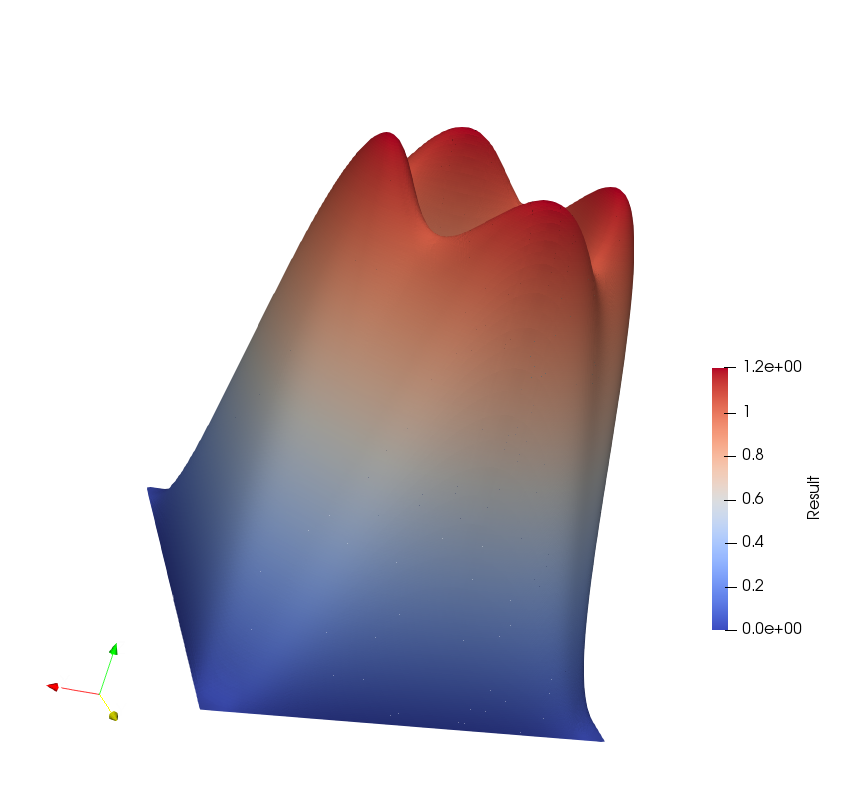
\includegraphics[width=10cm]{stokes_cg_velocities}
	\caption{The magnitude of the computed solution $\textbf{u}_h$ to problem (\ref{frame_stokes_disc}) with exact solution  $\left(\textbf{u},p\right)$ given by (\ref{benchmark_u}) and (\ref{benchmark_p}).}
	\label{fig_stokes_sol}
\end{figure}
\begin{table}[H]
	\begin{center}
		\begin{tabular}{|c|c|c|c|c|c|} \hline
			refinement cycle & cells & dofs & $||p-p_h||_{L^2}$ & $||u-u_h||_{L^2}$ & $||u-u_h||_{H^1}$\\ \hline
			0 & 64 & 679 & 5.1016e-02 & 1.0815e-02 & 4.4823e-01\\ \hline
			1 & 136 & 1431 & 1.0905e-01 & 9.9175e-03 & 4.1524e-01\\ \hline
			2 & 352 & 3635 & 9.7928e-02 & 7.1343e-03 & 2.9415e-01\\ \hline
			3 & 856 & 8615 & 2.3689e-02 & 9.6017e-04 & 8.2062e-02\\ \hline
			4 & 2128 & 21115 & 1.1988e-02 & 6.2091e-04 & 5.2756e-02\\ \hline
			5 & 5128 & 50427 & 2.4096e-03 & 8.6223e-05 & 1.5147e-02\\ \hline
		\end{tabular}
		\caption{Convergence for $\textbf{u}$ and $p$ in different norms for the simple Stokes model (for the first 5 refinement cycles).}
		\label{tablebenchmark_convergence}
	\end{center}
\end{table}


\begin{figure}[H]
	\begin{subfigure}[b]{.45\linewidth}
		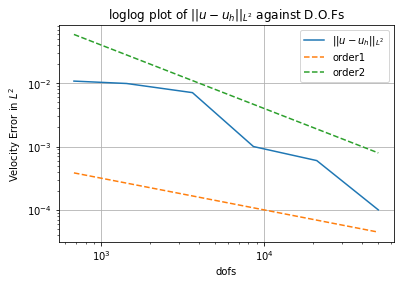
\includegraphics[width=\linewidth]{u_uh_L2}
		\caption{Velocity in $L^2$: $\left|\left|u-u_h\right|\right|_{L^2}$.}
		\label{fig_uL2}
	\end{subfigure}
	\begin{subfigure}[b]{.45\linewidth}
		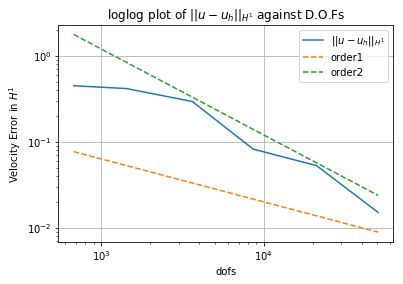
\includegraphics[width=\linewidth]{u_uh_H1}
		\caption{Velocity in $H^1$: $\left|\left|u-u_h\right|\right|_{H^1}$.}
		\label{fig_uH1}
	\end{subfigure}
	\centering
	\begin{subfigure}[b]{.45\linewidth}
		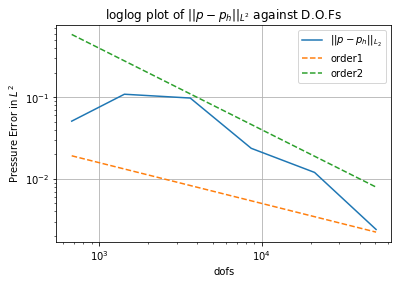
\includegraphics[width=\linewidth]{p_h_L2}
		\caption{Pressure $L^2$: $\left|\left|p-p_h\right|\right|_{L^2}$.}
		\label{fig_pL2}
	\end{subfigure}
	\caption{loglog plots of errors }
	\label{fig_errors}
\end{figure}
\subsubsection{Combined model with fixed interface}
Figures \ref{fig_combi_sol}  and \ref{fig_combi_sol_p} show surface plots of the magnitude of the computed solutions $\textbf{u}_h$  and $p_h$ respectively to problem (\ref{frame_combi_disc}) with exact solutions $\left(\textbf{u}, p\right)$ given by (\ref{benchmark_u_mm1}) and (\ref{benchmark_p_mm1}).
\begin{figure}[H]
	\centering
	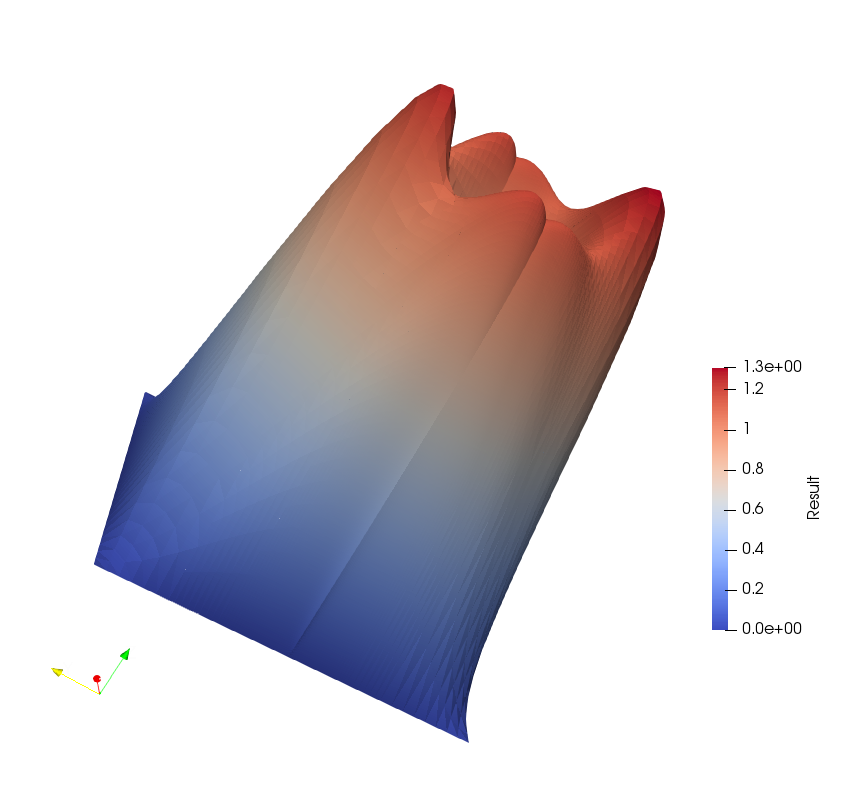
\includegraphics[width=10cm]{combi_u}
	\caption{The magnitude of the computed solution $\textbf{u}_h$ to problem (\ref{frame_combi_disc}) with exact solution $\left(\textbf{u},p\right)$ given by (\ref{benchmark_u_mm1}) and (\ref{benchmark_p_mm1}).}
	\label{fig_combi_sol}
\end{figure}
\begin{figure}[H]
	\centering
	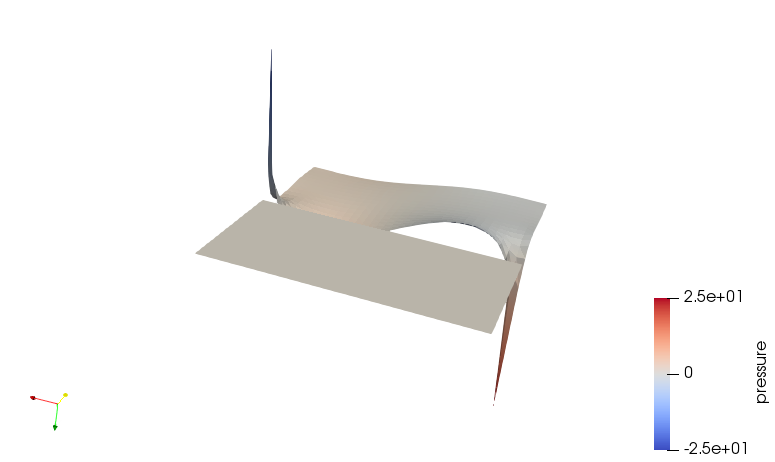
\includegraphics[width=10cm]{combi_p}
	\caption{The magnitude of the computed solution $p_h$ for problem (\ref{frame_combi_disc}) with exact solution $\left(\textbf{u},p\right)$ given by (\ref{benchmark_u_mm1}) and (\ref{benchmark_p_mm1}).}
	\label{fig_combi_sol_p}
\end{figure}
The convergence results are tabulated in Table \ref{tablebenchmark_convergence_mm1}.  
\begin{table}[H]
	\begin{center}
	\begin{tabular}{|c|c|c|c|c|c|} \hline
		refinement cycle & cells & dofs & $||p-p_h||_{L^2}$ & $||u-u_h||_{L^2}$ & $||u-u_h||_{Hdiv}$\\ \hline
		0 & 1024 & 20963 & 1.1118e+00 & 0.0964 & 0.4363\\ \hline
		1 & 2128 & 44039 & 1.1123e+00 & 0.0964 & 0.4360\\ \hline
		2 & 4408 & 91583 & 1.1125e+00 & 0.0964 & 0.4359\\ \hline
		3 & 9268 & 192207 & 1.1126e+00 & 0.0964 & 0.4359\\ \hline
		4 & 19480 & 403647 & 1.1126e+00 & 0.0964 & 0.4359\\ \hline
	\end{tabular}
		\caption{Convergence for $\textbf{u}$ and $p$ in different norms for the combined model with a fixed interface.}
		\label{tablebenchmark_convergence_mm1}
	\end{center}
\end{table}
\vspace{-10mm}

\subsection{Discussion}\label{sec_dealii_discussion}
The solution for the simple Stokes problem converges as we would expect for both velocity and pressure.  In contrast, for the combined problem both the velocity and the pressure do converge, but not to the solution we would expect given the right-hand side we have prescribed.   We can readily observe this by examining Figures \ref{fig_combi_sol} and \ref{fig_combi_sol_p} and comparing them with the prescribed data (\ref{benchmark_u_mm1}) and (\ref{benchmark_p_mm1}). 


Although the chosen pressure is in  $L^2_0\left(\Omega\right)$, $L^2_0\left(\Omega_S\right)$ and also $L^2_0\left(\mathcal{I}\right)$, this is not reflected in the computed solution.  We can see this from Figure \ref{fig_combi_sol}, where the jump in the gradient of the velocity across the interface is non-zero.  This is equivalent to sayng that the jump of the velocity gradient across the interface must integrate to something that is non-zero in order to balance the contribution from the pressure at the interface.  This should not be the case if the pressure was indeed in $L^2_0\left(\Omega_S\right)$ (and also in $L^2_0\left(\mathcal{I}\right)$ too). Furthermore, the pressure itself is not behaving according to the data we are prescribing in  (\ref{benchmark_u_mm1}) and (\ref{benchmark_p_mm1}), as we can see in Figure \ref{fig_combi_sol_p}.  It is attaining larger values than it should at the edges of the interface.  

A noteworthy feature of the results in Table \ref{tablebenchmark_convergence_mm1} is that, although we have convergence in both pressure and velocity in the $L^2$ norm, neither converges to what we would expect given the right hand side we prescribed.  We can see this as the error stabilizes but does not decrease.  Furthermore, the computed velocity solution is not divergenceless.




It has not been possible to accurately pinpoint the reason for this discrepancy.    However, it is noteworthy that this occurs most noticeably at the interface.  Recall that the interface condition in this case was prescribed such that the pressure would integrate to zero along the interface.  The intention behind this was that the jump in the velocity gradient across the interface would also integrate to zero.  This does not happen.  In fact, the solution is behaving as though there is a non-zero gradient jump across the interface.  

There are multiple possibilities for this behaviour.  It could be a bug in the code or of the analysis.  For example, the boundary conditions could be incompatible with the interface condition. 



\section{Concluding remarks and next steps}\label{sec_conclusion}
In this report we have shown the well-posedness of the combined Stokes-Laplace problem.  Furthermore, we have derived an a-posteriori indicator for the combined problem based on the abstract variational framework from \cite{verfurth2013posteriori}.  This indicator can drive both model and mesh-adaptivity.  It is based on the approach of \cite{giesselmann2017posteriori}, where the indicator is also built to drive both mesh and model adaptivity.  Lastly, we have created a model  for the combined problem in Deal.II with a fixed interface in order to test the indicator.  The model exhibited  behavior which was unexpected given the interface condition and the problem data we prescribed.  The next step would be to to find the reasons behind this behaviour.  

More specifically, the pressure attains values it should not be attaining at the points where our interface ($y=0.5$) intersects the boundary, where we prescribe homogeneous Dirichlet boundary conditions for the velocity.  The velocity also exhibits a jump in gradient across the interface.  The next step would be to see what the effect of the boundary conditions is on this bahaviour.  We need to carry out more tests, including varying the shape of the interface and see what happens when the interface has no contact with the boundary.  Another possibility is to multiply the second derivatives of the model by a parameter and let it go to zero, to see if this will eliminate the jump in the velocity-gradient.  

Once the reasons behind this behaviour are understood we can  take the project towards full model and mesh adaptiviy in three steps.  These are to firstly use the indicator just for mesh adaptivity, then just for model adaptivity and finally for both,  without fixing the interface.  The expectation from this indicator is to enable us to use the complex (Stokes) model in the parts of the domain where it is necessary while maintaining the computational expenses low by using the simpler (Laplace) model everywhere else.  If this is succesful then we can use the knowledge and rationale behind this project to more complex models with more direct applications to climate simulation.

%\noindent\begin{minipage}{\textwidth} %
%	\begin{minipage}{0.5\textwidth}
%		\centering
%		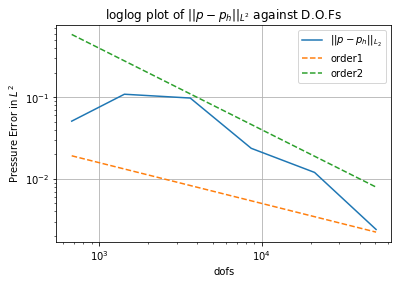
\includegraphics[width=.9\linewidth]{p_h_L2.png}
%		\captionof{subfigure}{caption}
%		\label{fig:figure1}
%	\end{minipage}
%	\begin{minipage}{0.5\textwidth}
%		\centering 
%		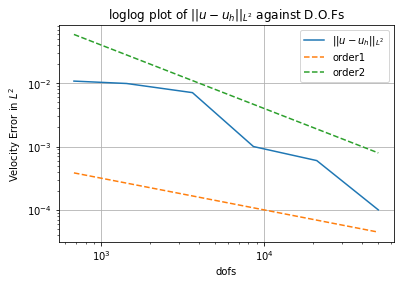
\includegraphics[width=.9\linewidth]{u_uh_L2.png} 
%		\captionof{subfigure}{caption} 
%		\label{fig:figure2} 
%	\end{minipage}\par
%	\begin{minipage}{0.5\textwidth}
%		\centering
%		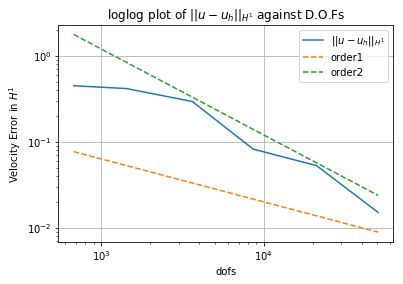
\includegraphics[width=.9\linewidth]{u_uh_H1.png}
%		\captionof{subfigure}{caption}
%		\label{fig:figure3}
%	\end{minipage}%
%	\captionof{figure}{figures} 
%	\label{fig:figures} 
%\end{minipage}
\bibliography{biblio_draft}
\bibliographystyle{ieeetr}
\end{document}